%-*-latex-*-
\documentclass[pdftex,12pt]{beamer}
\usepackage{etex,graphicx,pictex}
\setbeamercovered{transparent}
\begin{document}
%\title{Genetics and the Neolithic of Europe}
%\author{Alan R. Rogers}
%\date{7 Nov 2013}

%\frame{\titlepage}

\begin{frame}
\frametitle{Outline}
\begin{itemize}
\item The European Neolithic: a movement of peoples or of technology?
\item Linkage disequilibrium (LD)
\item How LD responds to changes in population size.
\item The history of European population size.
\end{itemize}
\end{frame}

\begin{frame}
\frametitle{Spread of farming across Europe}

\centering
  \includegraphics[height=0.8\textheight]{ClarkNeolith.png}\\
\hfill {\small (Grahame Clark, 1965, \emph{Proc.{} Prehist.{} Soc.})\\}
\end{frame}

\begin{frame}
\frametitle{Major axis of genetic variation in Europe}

\centering
  \includegraphics[width=\textwidth]{cavalli-pc1.jpeg}\\
\hfill {\small 95 genes (Cavalli-Sforza, 1994, p.~292)\\}
\end{frame}

\begin{frame}
\frametitle{Movement of people or of technology?}
  Local hunter-gatherers contributed less than 30\% in the original
  settlements. This finding leads us to reject a predominantly
  cultural transmission of agriculture.

\mbox{}\hfill\small(Loun{\`e}s Chikhi et al.{} 2002)

\vfill

Both mitochondrial DNA and Y chromosome analyses
have indicated a contribution of Neolithic Near Eastern lineages to
the gene pool of modern Europeans of around a quarter or less. This
suggests that dispersals bringing the Neolithic to Europe may have been
demographically minor. 

\mbox{}\hfill\small(Martin Richards 2003)
\end{frame}

%\begin{frame}
%\frametitle{24 ky old burial from Mal'ta, Siberia}
%
%\centering
%  \includegraphics[width=\textwidth]{malta.jpg}\\
%\hfill {\small (Willerslev \& Graf, forthcoming)\\}
%\end{frame}
%
%\begin{frame}
%\frametitle{24 ky old burial from Mal'ta, Siberia}
%\begin{columns}
%\column{0.5\textwidth}
%\includegraphics[width=\textwidth]{malta.jpg}\\
%\hfill {\small (Willerslev \& Graf, forthcoming)\\}
%\column{0.5\textwidth}
%\begin{itemize}
%\item $1/3$ of nuclear genome shared only with Native Americans
%\item mtDNA and Y chromosome shared only with Europeans
%\end{itemize}
%\end{columns}
%\end{frame}

\begin{frame}
\frametitle{Y haplogroup R1b1b2 most common in Ireland: Mesolithic origin?}

{\centering\includegraphics[height=0.8\textheight]{Balaresque-frq.pdf}\\}
\end{frame}

\begin{frame}
\frametitle{No: it originated in Turkey}

{\centering\includegraphics[width=\textwidth]{Balaresque-var.pdf}\\}
\end{frame}

\begin{frame}
\frametitle{Microsatellite variance vs. earliest Neolithic dates}

{\centering\includegraphics[height=0.75\textheight]{Balaresque-vxdate.pdf}\\}
\end{frame}

\begin{frame}
\frametitle{The Bl{\"a}tterh{\"o}hle site in Germany}

\centering
  \includegraphics[height=0.8\textheight]{Blatterhohle-map.png}\\
\end{frame}

\begin{frame}
\frametitle{mtDNA of Neolithic farmers and foragers}

\centering
  \includegraphics[height=0.8\textheight]{bollo1.png}\\
\hfill {\small (Bollongino et al, Oct 2013)\\}
\end{frame}

%\begin{frame}
%\frametitle{mtDNA of Neolithic farmers and foragers}
%
%\centering
%  \includegraphics[height=0.8\textheight]{bollo2.png}\\
%\hfill {\small (Bollongino et al, Oct 2013)\\}
%\end{frame}

\begin{frame}
\frametitle{Nuclear genes of Neolithic farmers and foragers}

\centering
  \includegraphics[width=\textwidth]{skoglund-struc.png}\\
\hfill {\small (Skoglund et al, 2012)\\}
\end{frame}

\begin{frame}
\frametitle{Nuclear genes of Neolithic farmers and foragers}

\centering
\includegraphics[height=0.8\textheight]{skoglund-pc.png}\\
\hfill {\small (Skoglund et al, 2012)\\}
\end{frame}

%\begin{frame}
%\frametitle{Northern Europeans resemble Neolithic foragers}
%
%\centering
%\includegraphics[height=0.7\textheight]{skoglund-forager.png}\\
%\hfill {\small (Skoglund et al, 2012)\\}
%\end{frame}
%
%\begin{frame}
%\frametitle{Southern Europeans resemble Neolithic farmers}
%
%\centering
%\includegraphics[height=0.7\textheight]{skoglund-farmer.png}\\
%\hfill {\small (Skoglund et al, 2012)\\}
%\end{frame}

\begin{frame}
\frametitle{Outline}
\begin{itemize}
\item[$\circ$] The European Neolithic: a movement of peoples or of technology?
\item Linkage disequilibrium (LD)
\item How LD responds to changes in population size.
\item The history of European population size.
\end{itemize}
\end{frame}

\begin{frame}
Linkage disequilibrium (LD) is one of those unfortunate terms that
does not reveal its meaning. As every instructor of population
genetics knows, the term is a barrier not an aid to
understanding\ldots Detecting LD does not ensure either linkage or a
lack of equilibrium.\\ \mbox{}\hfill\small(Montgomery Slatkin, 2008)
\end{frame}

\begin{frame}
\frametitle{Linkage disquilibrium (LD)}
\begin{columns}
\column{0.35\textwidth}
\centering
\begin{tabular}{ccc}
       & \multicolumn{2}{c}{Locus}\\
Gamete &  1 & 2\\ \hline
 1&A&B\\
 2&A&B\\
 3&A&B\\
 4&A&B\\
 5&A&B\\
 6&A&b\\
 7&a&B\\
 8&a&B\\
 9&a&b\\
10&a&b\\
\end{tabular}
\column{0.65\textwidth}
\pause
{\centering
\begin{tabular}{c|cc|c}
 \multicolumn{1}{c}{} & A & \multicolumn{1}{c}{a}\\
\cline{2-3}
B & 5 & 2 & 7\\
b & 1 & 2 & 3\\
\cline{2-3}
\multicolumn{1}{c}{} 
  & 6 & \multicolumn{1}{c}{4} & 10
\end{tabular}\\}
\begin{itemize}
\item $B$ is more common among $A$-gametes than $a$-gametes.
\item $A$ is more common among $B$-gametes than $b$-gametes.
\end{itemize}
\end{columns}
\end{frame}

\begin{frame}
\frametitle{Linkage equilibrium (LE)}
\begin{columns}
\column{0.35\textwidth}
\centering
\begin{tabular}{ccc}
       & \multicolumn{2}{c}{Locus}\\
Gamete &  1 & 2\\ \hline
 1&A&B\\
 2&A&B\\
 3&A&B\\
 4&A&B\\
 5&A&b\\
 6&A&b\\
 7&a&B\\
 8&a&B\\
 9&a&b\\
\end{tabular}
\column{0.65\textwidth}
{\centering
\begin{tabular}{c|cc|c}
 \multicolumn{1}{c}{} & A & \multicolumn{1}{c}{a}\\
\cline{2-3}
B & 4 & 2 & 6\\
b & 2 & 1 & 3\\
\cline{2-3}
\multicolumn{1}{c}{} 
  & 6 & \multicolumn{1}{c}{3} & 9
\end{tabular}\\}
\begin{itemize}
\item $B$ is equally common among $A$-gametes and $a$-gametes.
\item $A$ is equally common among $B$-gametes and $b$-gametes.
\end{itemize}
\end{columns}
\end{frame}

\begin{frame}
\frametitle{You can see LD in sequence data}
\begin{columns}
\column{0.6\textwidth}
 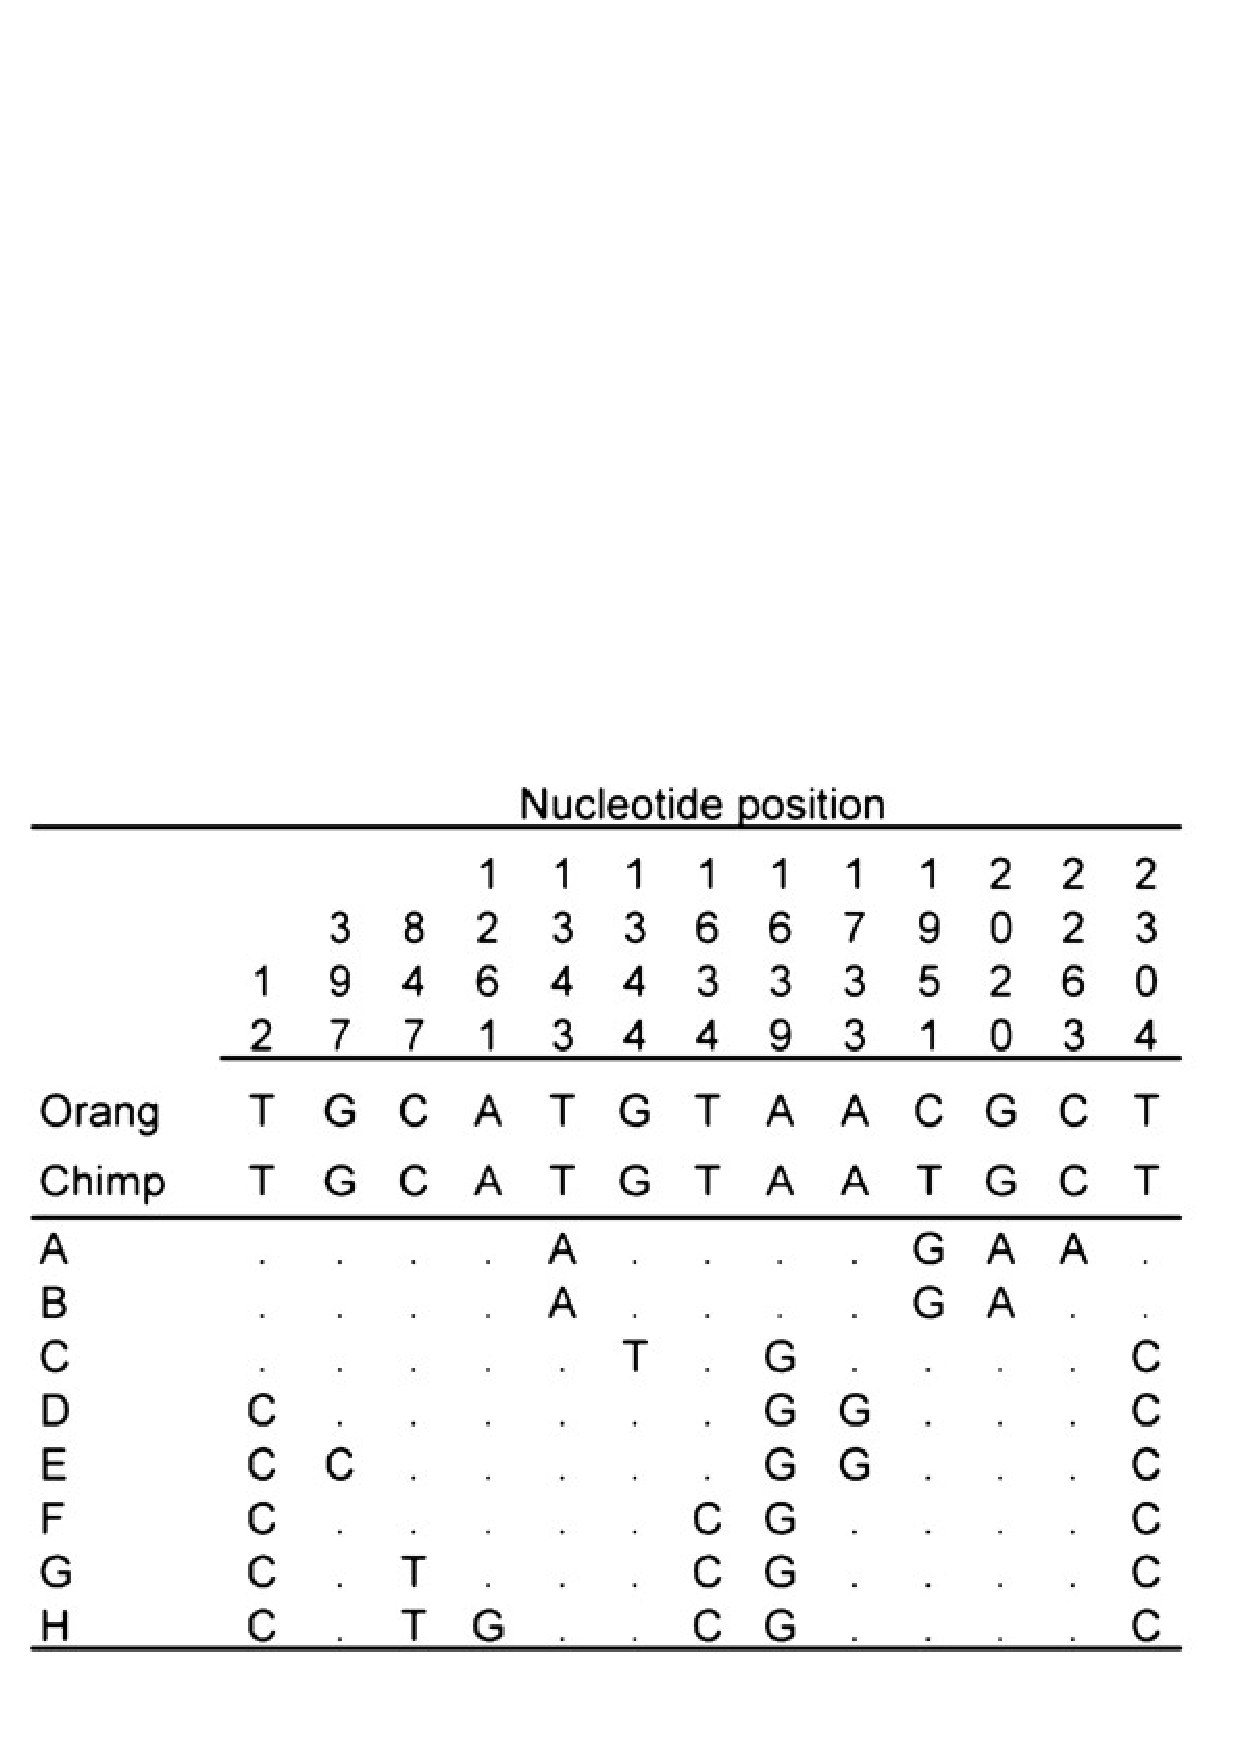
\includegraphics[width=\textwidth]{rrm2p4seq.png}\\
\textsc{\footnotesize (Garrigan et al 2004)}
\column{0.4\textwidth}\raggedright
\begin{itemize}
\item Dots: identical to chimp sequence.
\item Sites not independent.
\item A at site 1343 predicts G at 1951
\item This is linkage disequilibrium (LD).
\end{itemize}
\end{columns}
\end{frame}

\begin{frame}
\frametitle{Cross-overs shuffle DNA}
\begin{columns}
\column{0.6\textwidth}
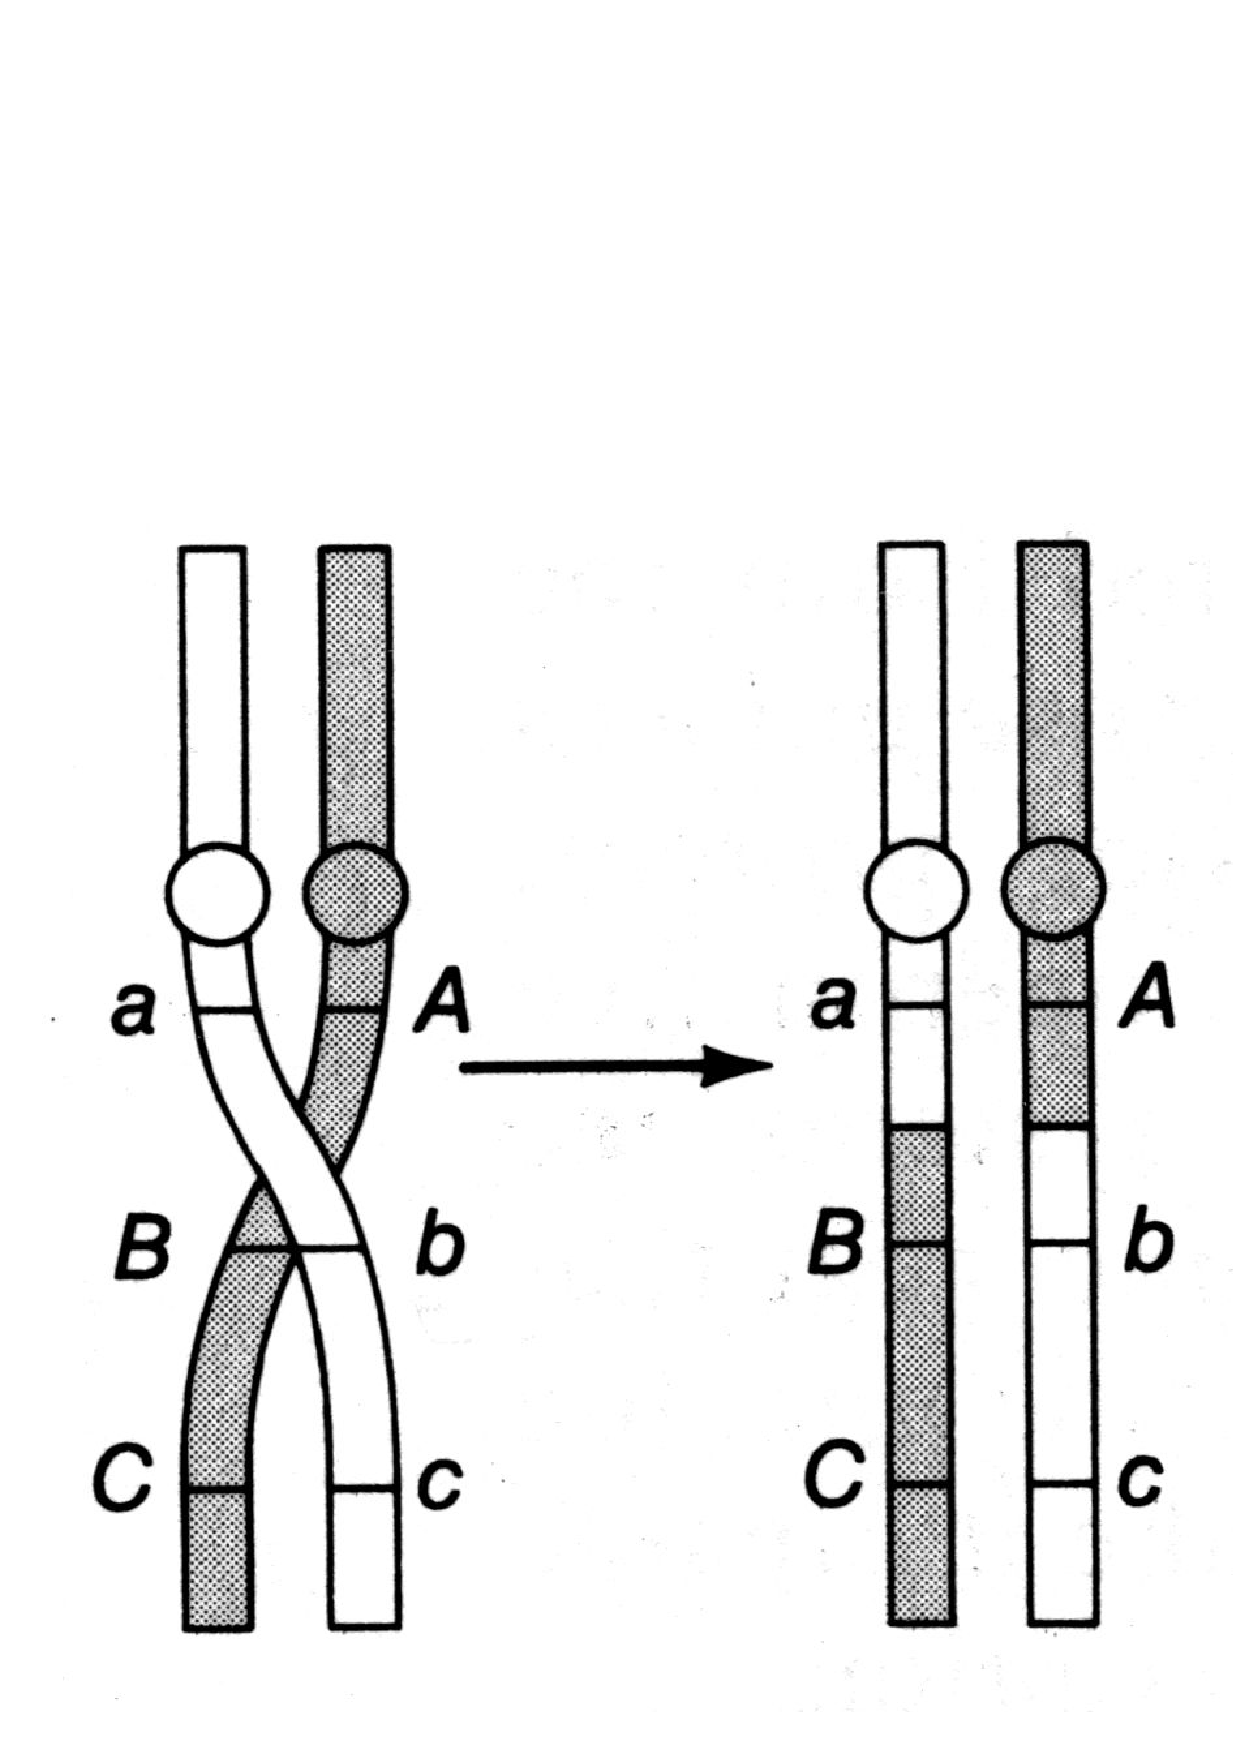
\includegraphics[width=\textwidth]{crossover.pdf}
\column{0.4\textwidth}
\raggedright
\begin{itemize}
\item occur during reproduction.
\item shuffle parental chromosomes.
\item sites far apart shuffled more.
\item destroys LD
\end{itemize}
\end{columns}
\end{frame}

\begin{frame}
\frametitle{Why population size affects LD}

\begin{itemize}
\item Small populations have short genealogies.
\item Little time for recombination to happen.
\item Lots of LD.
\end{itemize}
\end{frame}

\begin{frame}
\frametitle{Conventional measure of LD}
\[ 
D = P_{11} - a b 
\]
where $P_{11}$ is frequency of gamete type $A_1B_1$, $a$ is frequency
of allele~$A_1$ and $b$ is that of $B_1$.\\
\mbox{}\hfill{\small (Lewontin \& Kojima, 1960)\\}
\end{frame}

\begin{frame}
\frametitle{An alternative measure}
\[ \sigma_d^2 = \frac{E[D^2]}{E[a(1-a)b(1-b)]} \]
\mbox{}\hfill{\small (Ohta and Kimura, 1969)\\}
\begin{itemize}
\item Sensitive to loci with deep gene trees.
\item Allows us to see farther into the past.
\item Insensitive to sequencing error.
\item Deterministic theory relating $\sigma_d^2$ to population history.
\end{itemize}
\end{frame}

\begin{frame}
\frametitle{European LD curve for chromosome 1}
{\centering%auto-ignore
\mbox{\beginpicture
\setcoordinatesystem units <10in,18cm>
\setplotarea x from 0 to 0.3, y from 0 to 0.37
\axis left label {\large $\hat\sigma_d^2$} 
  ticks numbered from 0.0 to 0.3 by 0.1 /
\axis bottom label {\large Distance Between Sites (cM)}
  ticks numbered from 0.0 to 0.3 by 0.1 /
\put {\begin{tabular}{ll}
   circles & estimated $\sigma_d^2$\\
   dashes  & 95\% moving blocks bootstrap
   \end{tabular}} [rt] at 0.34 0.37
\multiput {$\circ$} at
%        cM      sigdsq
 0.00588908  0.34614516
 0.02218103  0.18678186
 0.03736414  0.13144474
 0.05240364  0.09366733
 0.06740198  0.07460503
 0.08249028  0.05841765
 0.09751629  0.04833787
 0.11242776  0.03978328
 0.12752425  0.03390208
 0.14246357  0.02777732
 0.15748250  0.02492866
 0.17245244  0.02233815
 0.18756300  0.02012957
 0.20257386  0.01859720
 0.21749347  0.01730525
 0.23250299  0.01594641
 0.24749493  0.01527014
 0.26252257  0.01498048
 0.27746795  0.01457843
 0.29247932  0.01373967
/
\setdashes
\setdashes
% Lower confidence interval on ceu chromosome 1
\plot
%        cM        low 
 0.00588908  0.33980371
 0.02218103  0.17482375
 0.03736414  0.12128268
 0.05240364  0.08664656
 0.06740198  0.06791843
 0.08249028  0.05305212
 0.09751629  0.04261601
 0.11242776  0.03548946
 0.12752425  0.03052865
 0.14246357  0.02552626
 0.15748250  0.02311394
 0.17245244  0.02066386
 0.18756300  0.01864097
 0.20257386  0.01699183
 0.21749347  0.01627360
 0.23250299  0.01463654
 0.24749493  0.01441146
 0.26252257  0.01411046
 0.27746795  0.01371537
 0.29247932  0.01286667
/
% Upper confidence interval on ceu chromosome 1
\plot
%        cM       high 
 0.00588908  0.36547230
 0.02218103  0.19766787
 0.03736414  0.14046946
 0.05240364  0.10031656
 0.06740198  0.08098384
 0.08249028  0.06475364
 0.09751629  0.05613984
 0.11242776  0.04610807
 0.12752425  0.03827509
 0.14246357  0.02961930
 0.15748250  0.02656523
 0.17245244  0.02388691
 0.18756300  0.02150364
 0.20257386  0.02046532
 0.21749347  0.01856236
 0.23250299  0.01744676
 0.24749493  0.01612734
 0.26252257  0.01584467
 0.27746795  0.01563822
 0.29247932  0.01463997
/
\endpicture}
\\}
\end{frame}

\begin{frame}
\frametitle{Outline}
\begin{itemize}
\item[$\circ$] The European Neolithic: a movement of peoples or of technology?
\item[$\circ$] Linkage disequilibrium (LD)
\item How LD responds to changes in population size.
\item The history of European population size.
\end{itemize}
\end{frame}

\begin{frame}
\frametitle{What does population growth do to the LD curve?}
{\centering\input{figgromodel}\\}

\bigskip

$t$ generations ago, the population $(2N)$ grew from $10^3$ to
$10^6$. 
\end{frame}

\begin{frame}
\frametitle{After population growth, right side delines fastest}
{\centering% y range: 0 to 0.1
\mbox{\beginpicture
%%%%%%%%%%%%%%%%%%%%%%%%%%%%%%%%%%%%%%%%%%%%%%%%%%%%%%%%%%%%%%%%
\setcoordinatesystem units <9in,0.68in>
\setplotarea x from 0 to 0.3, y from -4.2 to -0.5
\axis right label {$\sigma_d^2$}
  ticks withvalues 0.1 0.01 0.001 0.0001 /
  at -1 -2 -3 -4 / /
\axis bottom label {$100\times c$}
  ticks numbered from 0.0 to 0.3 by 0.1 /
\put {\small $t = \infty$} [r] <-4pt,02pt> at 0.01000000  -3.08032897
\plot
%       100c          eq0
  0.01000000  -3.08032897
  0.02450000  -3.25116972
  0.03900000  -3.37344368
  0.05350000  -3.46873451
  0.06800000  -3.54682256
  0.08250000  -3.61297789
  0.09700000  -3.67036749
  0.11150000  -3.72104400
  0.12600000  -3.76641404
  0.14050000  -3.80748378
  0.15500000  -3.84499781
  0.16950000  -3.87952267
  0.18400000  -3.91149942
  0.19850000  -3.94127817
  0.21300000  -3.96914149
  0.22750000  -3.99532074
  0.24200000  -4.02000774
  0.25650000  -4.04336328
  0.27100000  -4.06552351
  0.28550000  -4.08660469
/
\put {\small $t=0$} [r] <-4pt,0pt> at 0.01000000  -0.54815348
\plot
%       100c          eq1
  0.01000000  -0.54815348
  0.02450000  -0.61731953
  0.03900000  -0.67671217
  0.05350000  -0.72875147
  0.06800000  -0.77505873
  0.08250000  -0.81677297
  0.09700000  -0.85472482
  0.11150000  -0.88953852
  0.12600000  -0.92169500
  0.14050000  -0.95157259
  0.15500000  -0.97947421
  0.16950000  -1.00564615
  0.18400000  -1.03029136
  0.19850000  -1.05357904
  0.21300000  -1.07565169
  0.22750000  -1.09663050
  0.24200000  -1.11661936
  0.25650000  -1.13570799
  0.27100000  -1.15397444
  0.28550000  -1.17148701
/
\setsolid
\put {\small $t=500$} [r] <-4pt,0pt> at 0.01000000  -0.84942828
\plot
%       100c           s0
  0.01000000  -0.84942828
  0.02450000  -0.98399449
  0.03900000  -1.10802506
  0.05350000  -1.22419649
  0.06800000  -1.33427645
  0.08250000  -1.43949228
  0.09700000  -1.54072968
  0.11150000  -1.63864764
  0.12600000  -1.73374869
  0.14050000  -1.82642371
  0.15500000  -1.91698176
  0.16950000  -2.00566892
  0.18400000  -2.09268396
  0.19850000  -2.17818908
  0.21300000  -2.26231571
  0.22750000  -2.34517045
  0.24200000  -2.42683908
  0.25650000  -2.50738952
  0.27100000  -2.58687409
  0.28550000  -2.66533109
/
\put {\small $t=1000$} [r] <-4pt,0pt> at 0.01000000  -1.11136621
\plot
%       100c           s1
  0.01000000  -1.11136621
  0.02450000  -1.30962845
  0.03900000  -1.49679348
  0.05350000  -1.67560358
  0.06800000  -1.84781453
  0.08250000  -2.01458477
  0.09700000  -2.17667863
  0.11150000  -2.33457788
  0.12600000  -2.48854260
  0.14050000  -2.63864584
  0.15500000  -2.78478761
  0.16950000  -2.92669222
  0.18400000  -3.06393344
  0.19850000  -3.19592440
  0.21300000  -3.32194111
  0.22750000  -3.44116038
  0.24200000  -3.55272307
  0.25650000  -3.65582445
  0.27100000  -3.74982699
  0.28550000  -3.83432056
/
\put {\small $t=1500$} [r] <-4pt,0pt> at 0.01000000  -1.34556340
\plot
%       100c           s2
  0.01000000  -1.34556340
  0.02450000  -1.60611886
  0.03900000  -1.85456457
  0.05350000  -2.09326994
  0.06800000  -2.32336238
  0.08250000  -2.54503728
  0.09700000  -2.75767344
  0.11150000  -2.95985515
  0.12600000  -3.14942562
  0.14050000  -3.32368319
  0.15500000  -3.47983723
  0.16950000  -3.61559720
  0.18400000  -3.72998966
  0.19850000  -3.82371162
  0.21300000  -3.89895449
  0.22750000  -3.95881710
  0.24200000  -4.00661179
  0.25650000  -4.04537848
  0.27100000  -4.07740690
  0.28550000  -4.10459189
/
\put {\small $t=2000$} [r] <-4pt,0pt> at 0.01000000  -1.55899750
\plot
%       100c           s3
  0.01000000  -1.55899750
  0.02450000  -1.87986549
  0.03900000  -2.18592990
  0.05350000  -2.47766677
  0.06800000  -2.75314025
  0.08250000  -3.00809090
  0.09700000  -3.23641953
  0.11150000  -3.43171777
  0.12600000  -3.59002143
  0.14050000  -3.71204135
  0.15500000  -3.80303904
  0.16950000  -3.87050428
  0.18400000  -3.92151069
  0.19850000  -3.96159700
  0.21300000  -3.99461159
  0.22750000  -4.02299562
  0.24200000  -4.04826149
  0.25650000  -4.07134684
  0.27100000  -4.09285556
  0.28550000  -4.11297819
/
\endpicture}
\\}
\end{frame}

\begin{frame}
\frametitle{What does population decline do to the LD curve?}
{\centering% -*-latex-*-
\mbox{\beginpicture
\valuestolabelleading=.4\baselineskip
\setcoordinatesystem units <0.24in, 0.0018in> point at 0 0
\setplotarea x from 0 to 14, y from 0 to 500
\axis left shiftedto x=-0.5 label {$2N$}
  ticks  withvalues {$10^3$} {$10^6$} / at 1 500 / /
\axis bottom shiftedto y=-50
  label {Generations before present}
  ticks withvalues {$t$} / at 7 / /
\put{\em Assumed history} [rt] at 14 450
\plot 0 1 7 1 7 500 14 500 /
\endpicture}
\\}

\bigskip

$t$ generations ago, the population $(2N)$ shrank from $10^6$ to
$10^3$. 
\end{frame}

\begin{frame}
\frametitle{After population decline, whole curve rises}
{\centering\let\put\pictexput
\mbox{\beginpicture
%%%%%%%%%%%%%%%%%%%%%%%%%%%%%%%%%%%%%%%%%%%%%%%%%%%%%%%%%%%%%%%%
\setcoordinatesystem units <10in,14cm>
\setplotarea x from 0 to 0.3, y from 0 to 0.44
\axis left label {$\sigma_d^2$}
  ticks numbered from 0.0 to 0.4 by 0.1 /
\axis right invisible
  ticks length <0pt> withvalues {$t=0$} {$30$} {$90$} {$150$} 
  {$t=\infty$} / 
  at 0.001660928 0.028557630 0.068236861 0.094776554 0.117971478 / /
\axis bottom label {Distance Between Sites (cM)}
  ticks numbered from 0.0 to 0.3 by 0.1 /
\plot
%        cM         eq0 : t=infinity
0.007500000 0.423453863
0.022894737 0.371484794
0.038289474 0.331028708
0.053684211 0.298632209
0.069078947 0.272098265
0.084473684 0.249962423
0.099868421 0.231210910
0.115263158 0.215119606
0.130657895 0.201157465
0.146052632 0.188926159
0.161447368 0.178121039
0.176842105 0.168505109
0.192236842 0.159891227
0.207631579 0.152129636
0.223026316 0.145099072
0.238421053 0.138700284
0.253815789 0.132851255
0.269210526 0.127483612
0.284605263 0.122539899
0.300000000 0.117971478
/
\plot
%        cM         eq1 t=0
0.007500000 0.056551003
0.022894737 0.020557699
0.038289474 0.012582779
0.053684211 0.009068458
0.069078947 0.007089375
0.084473684 0.005819694
0.099868421 0.004935905
0.115263158 0.004285272
0.130657895 0.003786274
0.146052632 0.003391430
0.161447368 0.003071211
0.176842105 0.002806285
0.192236842 0.002583469
0.207631579 0.002393462
0.223026316 0.002229513
0.238421053 0.002086606
0.253815789 0.001960935
0.269210526 0.001849558
0.284605263 0.001750168
0.300000000 0.001660928
/
\setdashes
\plot
%        cM      sigdsq t=30
0.007500000 0.084726371
0.022894737 0.049215053
0.038289474 0.041285097
0.053684211 0.037725634
0.069078947 0.035667841
0.084473684 0.034303538
0.099868421 0.033316527
0.115263158 0.032557642
0.130657895 0.031947315
0.146052632 0.031439222
0.161447368 0.031004561
0.176842105 0.030624481
0.192236842 0.030286128
0.207631579 0.029980434
0.223026316 0.029700817
0.238421053 0.029442385
0.253815789 0.029201427
0.269210526 0.028975073
0.284605263 0.028761071
0.300000000 0.028557630
/
\plot
%        cM      sigdsq t=90
0.007500000 0.138796064
0.022894737 0.103314919
0.038289474 0.094684597
0.053684211 0.090292674
0.069078947 0.087364424
0.084473684 0.085120570
0.099868421 0.083256623
0.115263158 0.081628944
0.130657895 0.080160830
0.146052632 0.078807513
0.161447368 0.077541048
0.176842105 0.076343047
0.192236842 0.075200871
0.207631579 0.074105517
0.223026316 0.073050373
0.238421053 0.072030450
0.253815789 0.071041894
0.269210526 0.070081665
0.284605263 0.069147320
0.300000000 0.068236861
/
\plot
%        cM      sigdsq t150
0.007500000 0.190264154
0.022894737 0.153769803
0.038289474 0.143543358
0.053684211 0.137497483
0.069078947 0.132933430
0.084473684 0.129093480
0.099868421 0.125680649
0.115263158 0.122553858
0.130657895 0.119636878
0.146052632 0.116884435
0.161447368 0.114267589
0.176842105 0.111766697
0.192236842 0.109367742
0.207631579 0.107060283
0.223026316 0.104836249
0.238421053 0.102689199
0.253815789 0.100613846
0.269210526 0.098605748
0.284605263 0.096661094
0.300000000 0.094776554
/
\endpicture}
\let\put\latexput
\\}
\end{frame}

\begin{frame}
\frametitle{What does a ``bottleneck'' do to the LD curve?}
{\centering\input{figbtlmodel}\\}

\bigskip

$t$ generations ago, the population recovered from a
100-generation bottleneck.
\end{frame}

\begin{frame}
\frametitle{Bottleneck makes curve \emph{very} steep}
{\centering%auto-ignore
\mbox{\beginpicture
\setcoordinatesystem units <10in,38cm> point at 0.4 0
\setplotarea x from 0 to 0.3, y from 0 to 0.16
\axis left label {\large $\sigma_d^2$} 
  ticks numbered from 0.00 to 0.15 by 0.05 /
\axis bottom label {\large Distance Between Sites (cM)}
  ticks numbered from 0.0 to 0.3 by 0.1 /
\axis right invisible
  ticks length <0pt> withvalues {$t=\infty$} {$t=0$} / 
  at 0.011848280 0.083003277 / /
\plot
%        cM         eq1 : large population
0.007500000 0.066350362
0.022894737 0.030581153
0.038289474 0.022670051
0.053684211 0.019186184
0.069078947 0.017224950
0.084473684 0.015966999
0.099868421 0.015091509
0.115263158 0.014447057
0.130657895 0.013952841
0.146052632 0.013561807
0.161447368 0.013244694
0.176842105 0.012982351
0.192236842 0.012761714
0.207631579 0.012573572
0.223026316 0.012411237
0.238421053 0.012269740
0.253815789 0.012145311
0.269210526 0.012035037
0.284605263 0.011936633
0.300000000 0.011848280
/
\plot
%        cM          LD t=0
0.007500000 0.156665522
0.022894737 0.121252872
0.038289474 0.112468464
0.053684211 0.107884649
0.069078947 0.104754575
0.084473684 0.102307391
0.099868421 0.100241953
0.115263158 0.098416167
0.130657895 0.096754089
0.146052632 0.095211338
0.161447368 0.093760155
0.176842105 0.092382218
0.192236842 0.091064893
0.207631579 0.089799140
0.223026316 0.088578279
0.238421053 0.087397241
0.253815789 0.086252079
0.269210526 0.085139654
0.284605263 0.084057421
0.300000000 0.083003277
/
\setdashes
\put {100} [bl] at 0.269210526 0.054572952
\plot
%        cM          LD t=100
0.007500000 0.155056231
0.022894737 0.116940388
0.038289474 0.105606262
0.053684211 0.098624196
0.069078947 0.093240471
0.084473684 0.088677033
0.099868421 0.084625718
0.115263158 0.080937703
0.130657895 0.077530629
0.146052632 0.074354008
0.161447368 0.071374277
0.176842105 0.068567601
0.192236842 0.065916108
0.207631579 0.063405780
0.223026316 0.061025216
0.238421053 0.058764857
0.253815789 0.056616497
0.269210526 0.054572952
0.284605263 0.052627837
0.300000000 0.050775400
/
\put {500} [bl] at 0.099868421 0.046028592
\plot
%        cM          LD t=500
0.007500000 0.148904073
0.022894737 0.101653052
0.038289474 0.083025262
0.053684211 0.070304672
0.069078947 0.060479284
0.084473684 0.052551623
0.099868421 0.046028592
0.115263158 0.040605885
0.130657895 0.036070595
0.146052632 0.032262730
0.161447368 0.029056972
0.176842105 0.026352683
0.192236842 0.024067779
0.207631579 0.022134633
0.223026316 0.020497157
0.238421053 0.019108606
0.253815789 0.017929900
0.269210526 0.016928282
0.284605263 0.016076242
0.300000000 0.015350649
/
\put {1000} [bl] at 0.099868421 0.026351498
\plot
%        cM          LD t=1000
0.007500000 0.141817171
0.022894737 0.086303701
0.038289474 0.063253169
0.053684211 0.048665918
0.069078947 0.038620033
0.084473684 0.031489141
0.099868421 0.026351498
0.115263158 0.022615272
0.130657895 0.019878735
0.146052632 0.017861564
0.161447368 0.016365158
0.176842105 0.015247517
0.192236842 0.014406492
0.207631579 0.013768280
0.223026316 0.013279371
0.238421053 0.012900854
0.253815789 0.012604352
0.269210526 0.012369115
0.284605263 0.012179926
0.300000000 0.012025591
/
\plot
%        cM          LD t=1500
0.007500000 0.135345488
0.022894737 0.074280654
0.038289474 0.049971358
0.053684211 0.036200384
0.069078947 0.027820664
0.084473684 0.022564782
0.099868421 0.019200590
0.115263158 0.017007166
0.130657895 0.015548774
0.146052632 0.014557413
0.161447368 0.013866358
0.176842105 0.013370950
0.192236842 0.013004946
0.207631579 0.012726050
0.223026316 0.012506991
0.238421053 0.012329991
0.253815789 0.012183303
0.269210526 0.012059045
0.284605263 0.011951835
0.300000000 0.011857921
/
\plot
%        cM          LD t=2000
0.007500000 0.129434954
0.022894737 0.064861023
0.038289474 0.041046068
0.053684211 0.029015066
0.069078947 0.022480465
0.084473684 0.018778262
0.099868421 0.016596600
0.115263158 0.015253865
0.130657895 0.014386042
0.146052632 0.013794874
0.161447368 0.013370378
0.176842105 0.013050293
0.192236842 0.012798526
0.207631579 0.012593541
0.223026316 0.012422058
0.238421053 0.012275567
0.253815789 0.012148399
0.269210526 0.012036613
0.284605263 0.011937371
0.300000000 0.011848553
/
\endpicture}
\\}
\end{frame}

\begin{frame}
\frametitle{Effect of population history on LD curve}
\begin{itemize}
\item After growth, right side of curve falls fastest
\item After bottleneck, this effect is exaggerated
\item After population decline, curve rises but stays flat
\pause
\item We can use these principles to infer population history.
\end{itemize}
\end{frame}

\begin{frame}
\frametitle{Outline}
\begin{itemize}
\item[$\circ$] The European Neolithic: a movement of peoples or of technology?
\item[$\circ$] Linkage disequilibrium (LD)
\item[$\circ$] How LD responds to changes in population size.
\item The history of European population size.
\end{itemize}
\end{frame}

\begin{frame}
\frametitle{European LD curve is steep}
{\centering%auto-ignore
\mbox{\beginpicture
\setcoordinatesystem units <10in,18cm>
\setplotarea x from 0 to 0.3, y from 0 to 0.37
\axis left label {\large $\hat\sigma_d^2$} 
  ticks numbered from 0.0 to 0.3 by 0.1 /
\axis bottom label {\large Distance Between Sites (cM)}
  ticks numbered from 0.0 to 0.3 by 0.1 /
\put {Solid lines show equilibrium curves} [tr] at 0.35 0.3
\multiput {$\circ$} at
%        cM      sigdsq
 0.00588908  0.34614516
 0.02218103  0.18678186
 0.03736414  0.13144474
 0.05240364  0.09366733
 0.06740198  0.07460503
 0.08249028  0.05841765
 0.09751629  0.04833787
 0.11242776  0.03978328
 0.12752425  0.03390208
 0.14246357  0.02777732
 0.15748250  0.02492866
 0.17245244  0.02233815
 0.18756300  0.02012957
 0.20257386  0.01859720
 0.21749347  0.01730525
 0.23250299  0.01594641
 0.24749493  0.01527014
 0.26252257  0.01498048
 0.27746795  0.01457843
 0.29247932  0.01373967
/
\setdashes
% Lower confidence interval on ceu chromosome 1
\plot
%        cM        low 
 0.00588908  0.33980371
 0.02218103  0.17482375
 0.03736414  0.12128268
 0.05240364  0.08664656
 0.06740198  0.06791843
 0.08249028  0.05305212
 0.09751629  0.04261601
 0.11242776  0.03548946
 0.12752425  0.03052865
 0.14246357  0.02552626
 0.15748250  0.02311394
 0.17245244  0.02066386
 0.18756300  0.01864097
 0.20257386  0.01699183
 0.21749347  0.01627360
 0.23250299  0.01463654
 0.24749493  0.01441146
 0.26252257  0.01411046
 0.27746795  0.01371537
 0.29247932  0.01286667
/
% Upper confidence interval on ceu chromosome 1
\plot
%        cM       high 
 0.00588908  0.36547230
 0.02218103  0.19766787
 0.03736414  0.14046946
 0.05240364  0.10031656
 0.06740198  0.08098384
 0.08249028  0.06475364
 0.09751629  0.05613984
 0.11242776  0.04610807
 0.12752425  0.03827509
 0.14246357  0.02961930
 0.15748250  0.02656523
 0.17245244  0.02388691
 0.18756300  0.02150364
 0.20257386  0.02046532
 0.21749347  0.01856236
 0.23250299  0.01744676
 0.24749493  0.01612734
 0.26252257  0.01584467
 0.27746795  0.01563822
 0.29247932  0.01463997
/
\setsolid
\plot
%        cM          LD predld.5k
0.007500000 0.339743794
0.022894737 0.223208004
0.038289474 0.167818449
0.053684211 0.135364742
0.069078947 0.114005614
0.084473684 0.098863187
0.099868421 0.087557892
0.115263158 0.078789410
0.130657895 0.071786536
0.146052632 0.066062604
0.161447368 0.061295169
0.176842105 0.057262036
0.192236842 0.053805050
0.207631579 0.050808542
0.223026316 0.048185933
0.238421053 0.045871123
0.253815789 0.043812759
0.269210526 0.041970335
0.284605263 0.040311466
0.300000000 0.038809950
/
\plot
%        cM          LD predld.30k
0.007500000 0.151730335
0.022894737 0.069101775
0.038289474 0.047092685
0.053684211 0.036839418
0.069078947 0.030898126
0.084473684 0.027018541
0.099868421 0.024285218
0.115263158 0.022255148
0.130657895 0.020687679
0.146052632 0.019440774
0.161447368 0.018425170
0.176842105 0.017581941
0.192236842 0.016870621
0.207631579 0.016262491
0.223026316 0.015736609
0.238421053 0.015277342
0.253815789 0.014872783
0.269210526 0.014513705
0.284605263 0.014192844
0.300000000 0.013904407
/
\endpicture}
\\}
\end{frame}

\begin{frame}
\frametitle{3-parameter model of history}
{\centering% -*-latex-*-
\let\put\pictexput
\mbox{\beginpicture
\valuestolabelleading=.4\baselineskip
\setcoordinatesystem units <0.24in, 0.0018in> point at 0 0
\setplotarea x from 0 to 14, y from 0 to 500
\axis left shiftedto x=-0.5 
  ticks  withvalues {$2N_1$} {$2N_0$} / at 1 500 / /
\axis bottom shiftedto y=-50
  label {Generations before present}
  ticks withvalues {$t$} / at 7 / /
\put{\em Population Size} [rt] at 14 500
\plot 0 500 7 500 7 1 14 1 /
\endpicture}
\let\put\latexput
\\}

\bigskip

To estimate parameters, I search for values of $2N_0$, $2N_1$, and $t$
that provide best fit to observed LD curve.
\end{frame}

\begin{frame}
\frametitle{Estimates from simulation of expanded population}
{\centering\mbox{\beginpicture
\headingtoplotskip=-0.5ex
\setcoordinatesystem units <1cm,0.714cm> point at 2.5 2
\setplotarea x from 0 to 2.5, y from 2 to 8
\axis left label {\large $2N$} 
  ticks withvalues {$10^3$} {$10^4$} {$10^5$} {$10^6$} {$10^7$} / 
  at 3 4 5 6 7 / /
\axis bottom /
%
\put {$2N_0$} [b] at 1 7.5
\putrule from 1 4.2457 to 1 7.1628
\put {$\circ$} at 1 4.4542
\setdashes
\plot 0.5 6 1.5 6 /
\setsolid
%
\put {$2N_1$} [b] at 2 3.5
\putrule from 2 2.9408 to 2 3.0167
\put {$\circ$} at 2 2.9836
\setdashes
\plot 1.5 3 2.5 3 /
\setsolid
%%%%%%%%%%%%%%%%%%%%%%%%%%%%%%%%%%%%%%%%%%%%%%%%%%%%%%%%%%%%%%%%
\setcoordinatesystem units <1cm,0.0214cm> point at -0.5 200
\setplotarea x from 0 to 2, y from 200 to 400
\axis right label {\large $t$} 
  ticks numbered from 200 to 400 by 100 /
\axis bottom /
%
\put {$t_0$} [b] at 1 350
\putrule from 1 283.56 to 1 334.83
\put {$\circ$} at 1 314.01
\setdashes
\plot 0.5 300 1.5 300 /
\setsolid
\endpicture}
%
%# twoNinv0:     0.0005 3.5138e-05 (6.8736e-08,5.6794e-05)
%#    t0:       1000     314.01         (283.56,334.83)
%# twoNinv1:     0.0005  0.0010386   (0.00096238,0.001146)
%
%log10twoN0 = 4.4542 (4.2457,7.1628)
%log10twoN1 = 2.9836 (2.9408,3.0167)
\\}
Dashed lines show simulation parameters: $t_0=300$,
$2N_1=10^3$, and $2N_0=10^6$. Open circles
show parameter estimates, and vertical lines indicate 95\%
confidence intervals.
\end{frame}

\begin{frame}
\frametitle{Estimates from simulation of expanded population}
{\centering\let\put\pictexput
\mbox{\beginpicture
\headingtoplotskip=-0.5ex
\setcoordinatesystem units <0.0125cm,0.714cm> point at 0 1
\setplotarea x from 0 to 400, y from 1 to 8
\axis left label {\large $2N$} 
  ticks withvalues {$10^2$}  {$10^4$}  {$10^6$}  {$10^8$} / at 2 4 6 8 / /
\axis bottom label {Generations Ago} ticks numbered from 0 to 300 by 300 /
\plotheading{Expansion at $t=300$}
\setdots
\setdashes
\plot
%      t  logq0.25
   0.000   4.54799
  16.667   4.54799
  33.333   4.54799
  50.000   4.54799
  66.667   4.54799
  83.333   4.54799
 100.000   4.54799
 116.667   4.54799
 133.333   4.54799
 150.000   4.54799
 166.667   4.54799
 183.333   4.54799
 200.000   4.54799
 216.667   4.54799
 233.333   4.54799
 250.000   4.54799
 266.667   4.54799
 283.333   4.51939
 300.000   2.97127
 316.667   2.96573
 333.333   2.96508
 350.000   2.96508
 366.667   2.96508
 383.333   2.96508
 400.000   2.96508
/
\setsolid
\plot
%      t  logq0.5
   0.000  4.87983
  16.667  4.87983
  33.333  4.87983
  50.000  4.87983
  66.667  4.87983
  83.333  4.87983
 100.000  4.87983
 116.667  4.87983
 133.333  4.87983
 150.000  4.87983
 166.667  4.87983
 183.333  4.87983
 200.000  4.87983
 216.667  4.87983
 233.333  4.87983
 250.000  4.87983
 266.667  4.87983
 283.333  4.84080
 300.000  3.00218
 316.667  2.97909
 333.333  2.97783
 350.000  2.97783
 366.667  2.97783
 383.333  2.97783
 400.000  2.97783
/
\setdashes
\plot
%      t  logq0.75
   0.000   5.47354
  16.667   5.47354
  33.333   5.47354
  50.000   5.47354
  66.667   5.47354
  83.333   5.47354
 100.000   5.47354
 116.667   5.47354
 133.333   5.47354
 150.000   5.47354
 166.667   5.47354
 183.333   5.47354
 200.000   5.47354
 216.667   5.47354
 233.333   5.47354
 250.000   5.47354
 266.667   5.47354
 283.333   5.37661
 300.000   4.52166
 316.667   2.99739
 333.333   2.99122
 350.000   2.99120
 366.667   2.99120
 383.333   2.99120
 400.000   2.99120
/
\multiput {$\times$} at
000 6
050 6
100 6
150 6
200 6
250 6
300 6
300 3
350 3
400 3
/
\setsolid
\endpicture}
\let\put\latexput
%
%# twoNinv0:     0.0005 3.5138e-05 (6.8736e-08,5.6794e-05)
%#    t0:       1000     314.01         (283.56,334.83)
%# twoNinv1:     0.0005  0.0010386   (0.00096238,0.001146)
%
%log10twoN0 = 4.4542 (4.2457,7.1628)
%log10twoN1 = 2.9836 (2.9408,3.0167)
\\}
Shows same estimates as time path.
\end{frame}

\begin{frame}
\frametitle{Estimates from European chromosomes {\tiny(1000-Genomes Prj)}}
{\centering\let\put\pictexput
\mbox{\beginpicture
\headingtoplotskip=-0.5ex
%%%%%%%%%%%%%%% Begin Row 1 %%%%%%%%%%%%%%%%%%%%%%%%%%%%%%%%%%%%%%%%%%%%
\setcoordinatesystem units <0.005625cm,0.35cm> point at 0 1
\setplotarea x from 0 to 400, y from 1 to 8
\axis left label {\large $2N$} 
  ticks withvalues {$10^2$}  {$10^4$}  {$10^6$}  {$10^8$} / at 2 4 6 8 / /
\axis bottom 
  ticks unlabeled from 0 to 400 by 200 /
\plotheading{Chr 1}
\setdots
\setdashes
\plot
%      t  logq0.25
   0.000   6.01466
  16.667   6.01466
  33.333   6.01466
  50.000   6.01466
  66.667   6.01466
  83.333   6.01466
 100.000   6.01466
 116.667   6.01466
 133.333   6.01466
 150.000   6.01466
 166.667   6.01466
 183.333   6.01466
 200.000   6.01466
 216.667   6.01466
 233.333   6.00984
 250.000   5.96927
 266.667   4.07135
 283.333   3.68802
 300.000   3.67667
 316.667   3.67488
 333.333   3.67477
 350.000   3.67477
 366.667   3.67477
 383.333   3.67477
 400.000   3.67477
/
\setsolid
\plot
%      t   logq0.5
   0.000   6.47134
  16.667   6.47134
  33.333   6.47134
  50.000   6.47134
  66.667   6.47134
  83.333   6.47134
 100.000   6.47134
 116.667   6.47134
 133.333   6.47134
 150.000   6.47134
 166.667   6.47134
 183.333   6.47134
 200.000   6.47134
 216.667   6.47134
 233.333   6.47134
 250.000   6.44173
 266.667   6.14790
 283.333   3.71572
 300.000   3.69293
 316.667   3.68932
 333.333   3.68927
 350.000   3.68927
 366.667   3.68927
 383.333   3.68927
 400.000   3.68927
/
\setdashes
\plot
%      t  logq0.75
   0.000   7.05254
  16.667   7.05254
  33.333   7.05254
  50.000   7.05254
  66.667   7.05254
  83.333   7.05254
 100.000   7.05254
 116.667   7.05254
 133.333   7.05254
 150.000   7.05254
 166.667   7.05254
 183.333   7.05254
 200.000   7.05254
 216.667   7.05254
 233.333   7.05254
 250.000   7.04887
 266.667   6.83278
 283.333   6.10086
 300.000   3.71198
 316.667   3.70551
 333.333   3.70547
 350.000   3.70547
 366.667   3.70547
 383.333   3.70547
 400.000   3.70547
/
\setsolid
%%%%%%%%%%%%%%%%%%%%%%%%%%%%%%%%%%%%%%%%%%%%%%%%%%%%%%%%%%%%%%%%%%%%%%%%%%%
\setcoordinatesystem units <0.005625cm,0.35cm> point at -500 1
\setplotarea x from 0 to 400, y from 1 to 8
\axis left /
\axis bottom 
  ticks unlabeled from 0 to 400 by 200 /
\plotheading{Chr 2}
\setdots
\setdashes
\plot
%      t  logq0.25
   0.000   5.90488
  16.667   5.90488
  33.333   5.90488
  50.000   5.90488
  66.667   5.90488
  83.333   5.90488
 100.000   5.90488
 116.667   5.90488
 133.333   5.90488
 150.000   5.90488
 166.667   5.90488
 183.333   5.90488
 200.000   5.90488
 216.667   5.90488
 233.333   5.90488
 250.000   5.90488
 266.667   5.87920
 283.333   4.10739
 300.000   3.71515
 316.667   3.70778
 333.333   3.70629
 350.000   3.70564
 366.667   3.70564
 383.333   3.70564
 400.000   3.70564
/
\setsolid
\plot
%      t   logq0.5
   0.000   6.38127
  16.667   6.38127
  33.333   6.38127
  50.000   6.38127
  66.667   6.38127
  83.333   6.38127
 100.000   6.38127
 116.667   6.38127
 133.333   6.38127
 150.000   6.38127
 166.667   6.38127
 183.333   6.38127
 200.000   6.38127
 216.667   6.38127
 233.333   6.38127
 250.000   6.38127
 266.667   6.33863
 283.333   5.98212
 300.000   3.73257
 316.667   3.72103
 333.333   3.71959
 350.000   3.71924
 366.667   3.71924
 383.333   3.71924
 400.000   3.71924
/
\setdashes
\plot
%      t  logq0.75
   0.000   6.91942
  16.667   6.91942
  33.333   6.91942
  50.000   6.91942
  66.667   6.91942
  83.333   6.91942
 100.000   6.91942
 116.667   6.91942
 133.333   6.91942
 150.000   6.91942
 166.667   6.91942
 183.333   6.91942
 200.000   6.91942
 216.667   6.91942
 233.333   6.91942
 250.000   6.91942
 266.667   6.90630
 283.333   6.67853
 300.000   5.50279
 316.667   3.73657
 333.333   3.73311
 350.000   3.73251
 366.667   3.73251
 383.333   3.73251
 400.000   3.73251
/
\setsolid
%%%%%%%%%%%%%%%%%%%%%%%%%%%%%%%%%%%%%%%%%%%%%%%%%%%%%%%%%%%%%%%%%%%%%%%%%%%%
\setcoordinatesystem units <0.005625cm,0.35cm> point at -1000 1
\setplotarea x from 0 to 400, y from 1 to 8
\axis left /
\axis bottom 
  ticks unlabeled from 0 to 400 by 200 /
\plotheading{Chr 3}
\setdots
\setdashes
\plot
%      t  logq0.25
   0.000   4.09308
  16.667   4.09308
  33.333   4.09308
  50.000   4.09308
  66.667   4.09308
  83.333   4.09308
 100.000   4.09308
 116.667   4.09308
 133.333   4.09308
 150.000   4.09308
 166.667   4.09308
 183.333   4.09308
 200.000   4.09308
 216.667   4.09308
 233.333   4.09308
 250.000   4.08493
 266.667   3.74044
 283.333   3.70626
 300.000   3.70363
 316.667   3.70323
 333.333   3.70323
 350.000   3.70323
 366.667   3.70323
 383.333   3.70323
 400.000   3.70323
/
\setsolid
\plot
%      t   logq0.5
   0.000   6.08107
  16.667   6.08107
  33.333   6.08107
  50.000   6.08107
  66.667   6.08107
  83.333   6.08107
 100.000   6.08107
 116.667   6.08107
 133.333   6.08107
 150.000   6.08107
 166.667   6.08107
 183.333   6.08107
 200.000   6.08107
 216.667   6.08107
 233.333   6.08107
 250.000   5.97957
 266.667   4.08824
 283.333   3.73020
 300.000   3.72064
 316.667   3.72008
 333.333   3.72008
 350.000   3.72008
 366.667   3.72008
 383.333   3.72008
 400.000   3.72008
/
\setdashes
\plot
%      t  logq0.75
   0.000   6.70093
  16.667   6.70093
  33.333   6.70093
  50.000   6.70093
  66.667   6.70093
  83.333   6.70093
 100.000   6.70093
 116.667   6.70093
 133.333   6.70093
 150.000   6.70093
 166.667   6.70093
 183.333   6.70093
 200.000   6.70093
 216.667   6.70093
 233.333   6.70093
 250.000   6.66551
 266.667   6.30479
 283.333   4.07681
 300.000   4.05936
 316.667   4.05781
 333.333   4.05781
 350.000   4.05781
 366.667   4.05781
 383.333   4.05781
 400.000   4.05781
/
\setsolid
%%%%%%%%%%%%%%%%%%%%%%%%%%%%%%%%%%%%%%%%%%%%%%%%%%%%%%%%%%%%%%%%%%%%%%%%
%%%%%%%%%%%%%%% Begin Row 2 %%%%%%%%%%%%%%%%%%%%%%%%%%%%%%%%%%%%%%%%%%%%
%%%%%%%%%%%%%%%%%%%%%%%%%%%%%%%%%%%%%%%%%%%%%%%%%%%%%%%%%%%%%%%%%%%%%%%%
\setcoordinatesystem units <0.005625cm,0.35cm> point at  0 10.5
\setplotarea x from 0 to 400, y from 1 to 8
\axis left label {\large $2N$} 
  ticks withvalues {$10^2$}  {$10^4$}  {$10^6$}  {$10^8$} / at 2 4 6 8 / /
\axis bottom ticks numbered from 0 to 400 by 200 /
\plotheading{Chr 4}
\setdots
\setdashes
\plot
%      t  logq0.25
   0.000   4.07168
  16.667   4.07168
  33.333   4.07168
  50.000   4.07168
  66.667   4.07168
  83.333   4.07168
 100.000   4.07168
 116.667   4.07168
 133.333   4.07168
 150.000   4.07168
 166.667   4.07168
 183.333   4.07168
 200.000   4.07168
 216.667   4.07168
 233.333   4.07168
 250.000   4.07158
 266.667   4.06005
 283.333   3.69493
 300.000   3.68016
 316.667   3.67790
 333.333   3.67790
 350.000   3.67790
 366.667   3.67790
 383.333   3.67790
 400.000   3.67790
/
\setsolid
\plot
%      t  logq0.5
   0.000  5.98156
  16.667  5.98156
  33.333  5.98156
  50.000  5.98156
  66.667  5.98156
  83.333  5.98156
 100.000  5.98156
 116.667  5.98156
 133.333  5.98156
 150.000  5.98156
 166.667  5.98156
 183.333  5.98156
 200.000  5.98156
 216.667  5.98156
 233.333  5.98156
 250.000  5.97617
 266.667  5.44876
 283.333  4.05595
 300.000  3.70664
 316.667  3.70099
 333.333  3.70099
 350.000  3.70099
 366.667  3.70099
 383.333  3.70099
 400.000  3.70099
/
\setdashes
\plot
%      t logq0.75
   0.000  6.63586
  16.667  6.63586
  33.333  6.63586
  50.000  6.63586
  66.667  6.63586
  83.333  6.63586
 100.000  6.63586
 116.667  6.63586
 133.333  6.63586
 150.000  6.63586
 166.667  6.63586
 183.333  6.63586
 200.000  6.63586
 216.667  6.63586
 233.333  6.63586
 250.000  6.63586
 266.667  6.48032
 283.333  4.08498
 300.000  4.06321
 316.667  4.05935
 333.333  4.05935
 350.000  4.05935
 366.667  4.05935
 383.333  4.05935
 400.000  4.05935
/
\setsolid
%%%%%%%%%%%%%%%%%%%%%%%%%%%%%%%%%%%%%%%%%%%%%%%%%%%%%%%%%%%%%%%%
\setcoordinatesystem units <0.005625cm,0.35cm> point at -500 10.5
\setplotarea x from 0 to 400, y from 1 to 8
\axis left /
\axis bottom ticks numbered from 0 to 400 by 200 /
\plotheading{Chr 5}
\setdots
\setdashes
\plot
%      t  logq0.25
   0.000   5.85393
  16.667   5.85393
  33.333   5.85393
  50.000   5.85393
  66.667   5.85393
  83.333   5.85393
 100.000   5.85393
 116.667   5.85393
 133.333   5.85393
 150.000   5.85393
 166.667   5.85393
 183.333   5.85393
 200.000   5.85393
 216.667   5.85393
 233.333   5.84682
 250.000   5.76236
 266.667   3.71786
 283.333   3.68774
 300.000   3.67973
 316.667   3.67790
 333.333   3.67731
 350.000   3.67731
 366.667   3.67731
 383.333   3.67731
 400.000   3.67731
/
\setsolid
\plot
%      t   logq0.5
   0.000   6.37475
  16.667   6.37475
  33.333   6.37475
  50.000   6.37475
  66.667   6.37475
  83.333   6.37475
 100.000   6.37475
 116.667   6.37475
 133.333   6.37475
 150.000   6.37475
 166.667   6.37475
 183.333   6.37475
 200.000   6.37475
 216.667   6.37475
 233.333   6.37378
 250.000   6.32279
 266.667   5.92054
 283.333   3.70522
 300.000   3.69347
 316.667   3.69170
 333.333   3.69154
 350.000   3.69154
 366.667   3.69154
 383.333   3.69154
 400.000   3.69154
/
\setdashes
\plot
%      t  logq0.75
   0.000   6.97462
  16.667   6.97462
  33.333   6.97462
  50.000   6.97462
  66.667   6.97462
  83.333   6.97462
 100.000   6.97462
 116.667   6.97462
 133.333   6.97462
 150.000   6.97462
 166.667   6.97462
 183.333   6.97462
 200.000   6.97462
 216.667   6.97462
 233.333   6.97462
 250.000   6.90197
 266.667   6.59944
 283.333   5.48840
 300.000   3.70926
 316.667   3.70510
 333.333   3.70440
 350.000   3.70440
 366.667   3.70440
 383.333   3.70440
 400.000   3.70440
/
\setsolid
%%%%%%%%%%%%%%%%%%%%%%%%%%%%%%%%%%%%%%%%%%%%%%%%%%%%%%%%%%%%%%%%
\setcoordinatesystem units <0.005625cm,0.35cm> point at -1000 10.5
\setplotarea x from 0 to 400, y from 1 to 8
\axis left /
\axis bottom ticks numbered from 0 to 400 by 200 /
\plotheading{Chr 6}
\setdots
\setdashes
\plot
%      t  logq0.25
   0.000   3.99398
  16.667   3.99398
  33.333   3.99398
  50.000   3.99398
  66.667   3.99380
  83.333   3.99323
 100.000   3.99323
 116.667   3.99323
 133.333   3.99300
 150.000   3.99300
 166.667   3.99300
 183.333   3.99300
 200.000   3.99300
 216.667   3.99300
 233.333   3.99300
 250.000   3.99300
 266.667   3.99300
 283.333   3.99300
 300.000   3.99300
 316.667   3.99300
 333.333   3.99300
 350.000   3.99300
 366.667   3.99300
 383.333   3.99300
 400.000   3.99300
/
\setsolid
\plot
%      t   logq0.5
   0.000   4.01997
  16.667   4.01997
  33.333   4.01997
  50.000   4.01997
  66.667   4.01988
  83.333   4.01981
 100.000   4.01981
 116.667   4.01981
 133.333   4.01967
 150.000   4.01967
 166.667   4.01967
 183.333   4.01967
 200.000   4.01967
 216.667   4.01967
 233.333   4.01967
 250.000   4.01967
 266.667   4.01967
 283.333   4.01967
 300.000   4.01967
 316.667   4.01967
 333.333   4.01967
 350.000   4.01967
 366.667   4.01967
 383.333   4.01967
 400.000   4.01967
/
\setdashes
\plot
%      t  logq0.75
   0.000   4.03633
  16.667   4.03592
  33.333   4.03592
  50.000   4.03592
  66.667   4.03584
  83.333   4.03515
 100.000   4.03515
 116.667   4.03515
 133.333   4.03500
 150.000   4.03500
 166.667   4.03500
 183.333   4.03500
 200.000   4.03500
 216.667   4.03500
 233.333   4.03500
 250.000   4.03500
 266.667   4.03500
 283.333   4.03500
 300.000   4.03500
 316.667   4.03500
 333.333   4.03500
 350.000   4.03500
 366.667   4.03500
 383.333   4.03500
 400.000   4.03500
/
\setsolid
\endpicture}
\let\put\latexput
\\}
\end{frame}

\begin{frame}
\frametitle{Estimates from European chromosomes {\tiny(1000-Genomes Prj)}}
{\centering\let\put\pictexput
\mbox{\beginpicture
\headingtoplotskip=-0.5ex
%%%%%%%%%%%%%%%%%%%%%%%%%%%%%%%%%%%%%%%%%%%%%%%%%%%%%%%%%%%%%%%%%%%%%%%%%%%%%
\setcoordinatesystem units <0.005625cm,0.35cm> point at 0 1
\setplotarea x from 0 to 400, y from 1 to 8
\axis left label {\large $2N$} 
  ticks withvalues {$10^2$}  {$10^4$}  {$10^6$}  {$10^8$} / at 2 4 6 8 / /
\axis bottom 
  ticks unlabeled from 0 to 400 by 200 /
\plotheading{Chr 7}
\setdots
\setdashes
\plot
%      t  logq0.25
   0.000   5.33563
  16.667   5.33563
  33.333   5.33563
  50.000   5.33563
  66.667   5.33563
  83.333   5.33563
 100.000   5.33563
 116.667   5.33563
 133.333   5.33563
 150.000   5.33563
 166.667   5.30735
 183.333   5.28635
 200.000   5.24867
 216.667   5.14834
 233.333   4.46682
 250.000   3.90238
 266.667   3.86796
 283.333   3.83527
 300.000   3.80114
 316.667   3.78924
 333.333   3.78269
 350.000   3.78000
 366.667   3.77944
 383.333   3.77944
 400.000   3.77794
/
\setsolid
\plot
%      t   logq0.5
   0.000   5.84955
  16.667   5.84955
  33.333   5.84955
  50.000   5.84955
  66.667   5.84955
  83.333   5.84955
 100.000   5.84955
 116.667   5.84955
 133.333   5.84955
 150.000   5.84955
 166.667   5.83246
 183.333   5.82754
 200.000   5.78951
 216.667   5.73365
 233.333   5.56193
 250.000   5.21995
 266.667   4.56359
 283.333   3.89432
 300.000   3.85220
 316.667   3.83838
 333.333   3.83161
 350.000   3.82443
 366.667   3.82232
 383.333   3.82232
 400.000   3.82161
/
\setdashes
\plot
%      t  logq0.75
   0.000   6.53346
  16.667   6.53346
  33.333   6.53346
  50.000   6.53346
  66.667   6.53346
  83.333   6.53346
 100.000   6.53346
 116.667   6.53346
 133.333   6.53346
 150.000   6.53346
 166.667   6.52980
 183.333   6.52980
 200.000   6.49323
 216.667   6.43514
 233.333   6.27962
 250.000   6.08508
 266.667   5.85329
 283.333   5.23421
 300.000   3.96102
 316.667   3.90238
 333.333   3.88553
 350.000   3.87908
 366.667   3.87870
 383.333   3.87870
 400.000   3.87605
/
\setsolid
%%%%%%%%%%%%%%%%%%%%%%%%%%%%%%%%%%%%%%%%%%%%%%%%%%%%%%%%%%%%%%%%%%%%%%%%%%%%%%
\setcoordinatesystem units <0.005625cm,0.35cm> point at -500 1
\setplotarea x from 0 to 400, y from 1 to 8
\axis left /
\axis bottom 
  ticks unlabeled from 0 to 400 by 200 /
\plotheading{Chr 8}
\setdots
\setdashes
\plot
%      t  logq0.25
   0.000   4.04937
  16.667   4.04937
  33.333   4.04937
  50.000   4.04937
  66.667   4.04937
  83.333   4.04937
 100.000   4.04937
 116.667   4.04937
 133.333   4.04937
 150.000   4.04937
 166.667   4.04937
 183.333   4.04937
 200.000   4.04937
 216.667   4.04908
 233.333   4.04457
 250.000   4.02605
 266.667   3.71260
 283.333   3.70611
 300.000   3.70527
 316.667   3.70527
 333.333   3.70527
 350.000   3.70527
 366.667   3.70527
 383.333   3.70527
 400.000   3.70527
/
\setsolid
\plot
%      t   logq0.5
   0.000   4.06834
  16.667   4.06834
  33.333   4.06834
  50.000   4.06834
  66.667   4.06834
  83.333   4.06834
 100.000   4.06834
 116.667   4.06834
 133.333   4.06834
 150.000   4.06834
 166.667   4.06834
 183.333   4.06834
 200.000   4.06834
 216.667   4.06578
 233.333   4.06162
 250.000   4.05025
 266.667   4.04023
 283.333   4.03758
 300.000   4.03755
 316.667   4.03755
 333.333   4.03755
 350.000   4.03755
 366.667   4.03755
 383.333   4.03755
 400.000   4.03755
/
\setdashes
\plot
%      t  logq0.75
   0.000   6.01105
  16.667   6.01105
  33.333   6.01105
  50.000   6.01105
  66.667   6.01105
  83.333   6.01105
 100.000   6.01105
 116.667   6.01105
 133.333   6.01105
 150.000   6.01105
 166.667   6.01105
 183.333   6.01105
 200.000   6.01105
 216.667   5.97514
 233.333   5.84326
 250.000   4.06990
 266.667   4.05709
 283.333   4.05463
 300.000   4.05442
 316.667   4.05442
 333.333   4.05442
 350.000   4.05442
 366.667   4.05442
 383.333   4.05442
 400.000   4.05442
/
\setsolid
%%%%%%%%%%%%%%%%%%%%%%%%%%%%%%%%%%%%%%%%%%%%%%%%%%%%%%%%%%%%%%%%%%%%%%%%%%%%%%%
\setcoordinatesystem units <0.005625cm,0.35cm> point at -1000 1
\setplotarea x from 0 to 400, y from 1 to 8
\axis left /
\axis bottom ticks unlabeled from 0 to 400 by 200 /
\plotheading{Chr 9}
\setdots
\setdashes
\plot
%      t  logq0.25
   0.000   5.69318
  16.667   5.69318
  33.333   5.69318
  50.000   5.69318
  66.667   5.69318
  83.333   5.69318
 100.000   5.69318
 116.667   5.69318
 133.333   5.69318
 150.000   5.69318
 166.667   5.69318
 183.333   5.69318
 200.000   5.69318
 216.667   5.68271
 233.333   5.67186
 250.000   5.48979
 266.667   3.72595
 283.333   3.69230
 300.000   3.68178
 316.667   3.67478
 333.333   3.67270
 350.000   3.67232
 366.667   3.67228
 383.333   3.67194
 400.000   3.67194
/
\setsolid
\plot
%      t   logq0.5
   0.000   6.19635
  16.667   6.19635
  33.333   6.19635
  50.000   6.19635
  66.667   6.19635
  83.333   6.19635
 100.000   6.19635
 116.667   6.19635
 133.333   6.19635
 150.000   6.19635
 166.667   6.19635
 183.333   6.19635
 200.000   6.19635
 216.667   6.18647
 233.333   6.15973
 250.000   6.02097
 266.667   5.64843
 283.333   3.72585
 300.000   3.70429
 316.667   3.69499
 333.333   3.69367
 350.000   3.69313
 366.667   3.69312
 383.333   3.69306
 400.000   3.69306
/
\setdashes
\plot
%      t  logq0.75
   0.000   6.75549
  16.667   6.75549
  33.333   6.75549
  50.000   6.75549
  66.667   6.75549
  83.333   6.75549
 100.000   6.75549
 116.667   6.75549
 133.333   6.75549
 150.000   6.75549
 166.667   6.75549
 183.333   6.75549
 200.000   6.75549
 216.667   6.75513
 233.333   6.72165
 250.000   6.66814
 266.667   6.40015
 283.333   5.76238
 300.000   3.73837
 316.667   3.71834
 333.333   3.71639
 350.000   3.71541
 366.667   3.71540
 383.333   3.71488
 400.000   3.71488
/
\setsolid
%%%%%%%%%%%%%%%%%%%%%%%%%%%%%%%%%%%%%%%%%%%%%%%%%%%%%%%%%%%%%%%%
\setcoordinatesystem units <0.005625cm,0.35cm> point at 0 10.5
\setplotarea x from 0 to 400, y from 1 to 8
\axis left label {\large $2N$} 
  ticks withvalues {$10^2$}  {$10^4$}  {$10^6$}  {$10^8$} / at 2 4 6 8 / /
\axis bottom ticks numbered from 0 to 400 by 200 /
\plotheading{Chr 10}
\setdots
\setdashes
\plot
%      t  logq0.25
%      t  logq0.25
   0.000   5.78290
  16.667   5.78290
  33.333   5.78290
  50.000   5.78290
  66.667   5.78290
  83.333   5.78290
 100.000   5.78290
 116.667   5.78290
 133.333   5.78290
 150.000   5.78290
 166.667   5.78290
 183.333   5.78290
 200.000   5.78290
 216.667   5.78290
 233.333   5.78090
 250.000   5.74564
 266.667   5.64095
 283.333   3.73822
 300.000   3.69861
 316.667   3.68750
 333.333   3.68077
 350.000   3.67878
 366.667   3.67866
 383.333   3.67866
 400.000   3.67847
/
\setsolid
\plot
%      t   logq0.5
%      t   logq0.5
   0.000   6.22066
  16.667   6.22066
  33.333   6.22066
  50.000   6.22066
  66.667   6.22066
  83.333   6.22066
 100.000   6.22066
 116.667   6.22066
 133.333   6.22066
 150.000   6.22066
 166.667   6.22066
 183.333   6.22066
 200.000   6.22066
 216.667   6.22066
 233.333   6.22066
 250.000   6.21524
 266.667   6.14552
 283.333   5.76737
 300.000   3.73178
 316.667   3.71068
 333.333   3.70490
 350.000   3.70250
 366.667   3.70243
 383.333   3.70243
 400.000   3.70238
/
\setdashes
\plot
%      t  logq0.75
%      t  logq0.75
   0.000   6.82191
  16.667   6.82191
  33.333   6.82191
  50.000   6.82191
  66.667   6.82191
  83.333   6.82191
 100.000   6.82191
 116.667   6.82191
 133.333   6.82191
 150.000   6.82191
 166.667   6.82191
 183.333   6.82191
 200.000   6.82191
 216.667   6.82191
 233.333   6.82191
 250.000   6.79399
 266.667   6.72371
 283.333   6.47358
 300.000   5.62637
 316.667   3.73822
 333.333   3.73054
 350.000   3.72534
 366.667   3.72475
 383.333   3.72475
 400.000   3.72469
/
\setsolid
%%%%%%%%%%%%%%%%%%%%%%%%%%%%%%%%%%%%%%%%%%%%%%%%%%%%%%%%%%%%%%%%%%%%%%%%
\setcoordinatesystem units <0.005625cm,0.35cm> point at -500 10.5
\setplotarea x from 0 to 400, y from 1 to 8
\axis left /
\axis bottom ticks numbered from 0 to 400 by 200 /
\plotheading{Chr 11}
\setdots
\setdashes
\plot
%      t  logq0.25
%      t  logq0.25
   0.000   5.24802
  16.667   5.24802
  33.333   5.24802
  50.000   5.24802
  66.667   5.24802
  83.333   5.24802
 100.000   5.24802
 116.667   5.24802
 133.333   5.24802
 150.000   5.24802
 166.667   5.24802
 183.333   5.24802
 200.000   5.24802
 216.667   5.23101
 233.333   5.18018
 250.000   4.91143
 266.667   4.32877
 283.333   3.74589
 300.000   3.72746
 316.667   3.71872
 333.333   3.71457
 350.000   3.71241
 366.667   3.71073
 383.333   3.70865
 400.000   3.70829
/
\setsolid
\plot
%      t   logq0.5
%      t   logq0.5
   0.000   5.88969
  16.667   5.88969
  33.333   5.88969
  50.000   5.88969
  66.667   5.88969
  83.333   5.88969
 100.000   5.88969
 116.667   5.88969
 133.333   5.88969
 150.000   5.88969
 166.667   5.88969
 183.333   5.88969
 200.000   5.88969
 216.667   5.88328
 233.333   5.87110
 250.000   5.74350
 266.667   5.32636
 283.333   4.47025
 300.000   3.75862
 316.667   3.74589
 333.333   3.74178
 350.000   3.73970
 366.667   3.73836
 383.333   3.73646
 400.000   3.73555
/
\setdashes
\plot
%      t  logq0.75
%      t  logq0.75
   0.000   6.49148
  16.667   6.49148
  33.333   6.49148
  50.000   6.49148
  66.667   6.49148
  83.333   6.49148
 100.000   6.49148
 116.667   6.49148
 133.333   6.49148
 150.000   6.49148
 166.667   6.49148
 183.333   6.49148
 200.000   6.49148
 216.667   6.49148
 233.333   6.48443
 250.000   6.38622
 266.667   6.11197
 283.333   5.54383
 300.000   4.61864
 316.667   3.81969
 333.333   3.78133
 350.000   3.77600
 366.667   3.77205
 383.333   3.76752
 400.000   3.76564
/
\setsolid
%%%%%%%%%%%%%%%%%%%%%%%%%%%%%%%%%%%%%%%%%%%%%%%%%%%%%%%%%%%%%%%%%%%%%%%%%%%%%%%%
\setcoordinatesystem units <0.005625cm,0.35cm> point at -1000 10.5
\setplotarea x from 0 to 400, y from 1 to 8
\axis left /
\axis bottom ticks numbered from 0 to 400 by 200 /
\plotheading{Chr 12}
\setdashes
\plot
%      t  logq0.25
   0.000   5.38435
  16.667   5.38435
  33.333   5.38435
  50.000   5.38435
  66.667   5.38435
  83.333   5.38435
 100.000   5.38435
 116.667   5.37986
 133.333   5.37201
 150.000   5.29943
 166.667   5.09200
 183.333   4.76811
 200.000   3.70945
 216.667   3.67096
 233.333   3.64497
 250.000   3.62552
 266.667   3.60731
 283.333   3.59302
 300.000   3.57489
 316.667   3.56278
 333.333   3.55536
 350.000   3.55381
 366.667   3.54886
 383.333   3.54886
 400.000   3.54787
/
\setsolid
\plot
%      t   logq0.5
   0.000   5.89465
  16.667   5.89465
  33.333   5.89465
  50.000   5.89465
  66.667   5.89465
  83.333   5.89465
 100.000   5.89465
 116.667   5.89351
 133.333   5.89237
 150.000   5.86431
 166.667   5.75506
 183.333   5.60241
 200.000   5.27680
 216.667   4.68203
 233.333   3.70682
 250.000   3.68032
 266.667   3.65970
 283.333   3.64827
 300.000   3.63569
 316.667   3.62724
 333.333   3.62461
 350.000   3.62255
 366.667   3.61936
 383.333   3.61936
 400.000   3.61829
/
\setdashes
\plot
%      t  logq0.75
   0.000   6.44393
  16.667   6.44393
  33.333   6.44393
  50.000   6.44393
  66.667   6.44393
  83.333   6.44393
 100.000   6.44393
 116.667   6.44393
 133.333   6.43742
 150.000   6.42165
 166.667   6.33864
 183.333   6.25248
 200.000   6.06199
 216.667   5.83997
 233.333   5.47894
 250.000   4.81361
 266.667   3.74217
 283.333   3.71085
 300.000   3.68976
 316.667   3.68186
 333.333   3.67557
 350.000   3.67149
 366.667   3.66864
 383.333   3.66864
 400.000   3.66763
/
\endpicture}
\let\put\latexput
\\}
\end{frame}

\begin{frame}
\frametitle{Estimates from European chromosomes {\tiny(1000-Genomes Prj)}}
{\centering\mbox{\beginpicture
\headingtoplotskip=-0.5ex
%%%%%%%%%%%%%%%%%%%%%%%%%%%%%%%%%%%%%%%%%%%%%%%%%%%%%%%%%%%%%%%%%%%%%%%%%%%%%%%%
\setcoordinatesystem units <0.005625cm,0.35cm> point at 0 1
\setplotarea x from 0 to 400, y from 1 to 8
\axis left label {\large $2N$} 
  ticks withvalues {$10^2$}  {$10^4$}  {$10^6$}  {$10^8$} / at 2 4 6 8 / /
\axis bottom ticks unlabeled from 0 to 400 by 200 /
\plotheading{Chr 13}
\setdots
\setdashes
\plot
%      t  logq0.25
   0.000   5.76795
  16.667   5.76795
  33.333   5.76795
  50.000   5.76795
  66.667   5.76795
  83.333   5.76795
 100.000   5.76795
 116.667   5.76795
 133.333   5.76795
 150.000   5.76795
 166.667   5.76795
 183.333   5.76795
 200.000   5.76795
 216.667   5.76795
 233.333   5.76795
 250.000   5.75826
 266.667   5.59697
 283.333   3.74602
 300.000   3.71251
 316.667   3.70037
 333.333   3.69886
 350.000   3.69788
 366.667   3.69733
 383.333   3.69705
 400.000   3.69705
/
\setsolid
\plot
%      t  logq0.5
   0.000  6.21362
  16.667  6.21362
  33.333  6.21362
  50.000  6.21362
  66.667  6.21362
  83.333  6.21362
 100.000  6.21362
 116.667  6.21362
 133.333  6.21362
 150.000  6.21362
 166.667  6.21362
 183.333  6.21362
 200.000  6.21362
 216.667  6.21362
 233.333  6.21362
 250.000  6.20684
 266.667  6.13856
 283.333  5.84312
 300.000  3.74386
 316.667  3.72135
 333.333  3.71726
 350.000  3.71605
 366.667  3.71556
 383.333  3.71496
 400.000  3.71496
/
\setdashes
\plot
%      t logq0.75
   0.000  6.88287
  16.667  6.88287
  33.333  6.88287
  50.000  6.88287
  66.667  6.88287
  83.333  6.88287
 100.000  6.88287
 116.667  6.88287
 133.333  6.88287
 150.000  6.88287
 166.667  6.88287
 183.333  6.88287
 200.000  6.88287
 216.667  6.88287
 233.333  6.88287
 250.000  6.87846
 266.667  6.80133
 283.333  6.49368
 300.000  5.89208
 316.667  3.75079
 333.333  3.73999
 350.000  3.73874
 366.667  3.73743
 383.333  3.73572
 400.000  3.73572
/
\setsolid
%%%%%%%%%%%%%%%%%%%%%%%%%%%%%%%%%%%%%%%%%%%%%%%%%%%%%%%%%%%%%%%%%%%%%%%%%%%%%%%%
\setcoordinatesystem units <0.005625cm,0.35cm> point at -500 1
\setplotarea x from 0 to 400, y from 1 to 8
\axis left /
\axis bottom ticks unlabeled from 0 to 400 by 200 /
\plotheading{Chr 14}
\setdots
\setdashes
\plot
%      t logq0.25
   0.000  5.70651
  16.667  5.70651
  33.333  5.70651
  50.000  5.70651
  66.667  5.70651
  83.333  5.70651
 100.000  5.70651
 116.667  5.70651
 133.333  5.70651
 150.000  5.70651
 166.667  5.70651
 183.333  5.70651
 200.000  5.70651
 216.667  5.70651
 233.333  5.70651
 250.000  5.70156
 266.667  5.65791
 283.333  5.35690
 300.000  3.74432
 316.667  3.72213
 333.333  3.71486
 350.000  3.71321
 366.667  3.71275
 383.333  3.71275
 400.000  3.71269
/
\setsolid
\plot
%      t  logq0.5
   0.000  6.21394
  16.667  6.21394
  33.333  6.21394
  50.000  6.21394
  66.667  6.21394
  83.333  6.21394
 100.000  6.21394
 116.667  6.21394
 133.333  6.21394
 150.000  6.21394
 166.667  6.21394
 183.333  6.21394
 200.000  6.21394
 216.667  6.21394
 233.333  6.21394
 250.000  6.20833
 266.667  6.16585
 283.333  5.94236
 300.000  3.78677
 316.667  3.74076
 333.333  3.73249
 350.000  3.73091
 366.667  3.73037
 383.333  3.73037
 400.000  3.73024
/
\setdashes
\plot
%      t  logq0.75
   0.000   6.83544
  16.667   6.83544
  33.333   6.83544
  50.000   6.83544
  66.667   6.83544
  83.333   6.83544
 100.000   6.83544
 116.667   6.83544
 133.333   6.83544
 150.000   6.83544
 166.667   6.83544
 183.333   6.83544
 200.000   6.83544
 216.667   6.83544
 233.333   6.83544
 250.000   6.82006
 266.667   6.80645
 283.333   6.63904
 300.000   6.00021
 316.667   3.77021
 333.333   3.75199
 350.000   3.74853
 366.667   3.74816
 383.333   3.74816
 400.000   3.74796
/
\setsolid
%%%%%%%%%%%%%%%%%%%%%%%%%%%%%%%%%%%%%%%%%%%%%%%%%%%%%%%%%%%%%%%%%%%%%%%%%
\setcoordinatesystem units <0.005625cm,0.35cm> point at -1000 1
\setplotarea x from 0 to 400, y from 1 to 8
\axis left /
\axis bottom ticks unlabeled from 0 to 400 by 200 /
\plotheading{Chr 15}
\setdots
\setdashes
\plot
%      t logq0.25
   0.000  5.87376
  16.667  5.87376
  33.333  5.87376
  50.000  5.87376
  66.667  5.87376
  83.333  5.87376
 100.000  5.87376
 116.667  5.87376
 133.333  5.87376
 150.000  5.87376
 166.667  5.87376
 183.333  5.87376
 200.000  5.87376
 216.667  5.87376
 233.333  5.86496
 250.000  5.76262
 266.667  3.67573
 283.333  3.64492
 300.000  3.63796
 316.667  3.63723
 333.333  3.63723
 350.000  3.63723
 366.667  3.63723
 383.333  3.63723
 400.000  3.63723
/
\setsolid
\plot
%      t  logq0.5
   0.000  6.37518
  16.667  6.37518
  33.333  6.37518
  50.000  6.37518
  66.667  6.37518
  83.333  6.37518
 100.000  6.37518
 116.667  6.37518
 133.333  6.37518
 150.000  6.37518
 166.667  6.37518
 183.333  6.37518
 200.000  6.37518
 216.667  6.37518
 233.333  6.36573
 250.000  6.26494
 266.667  5.81051
 283.333  3.66372
 300.000  3.65421
 316.667  3.65328
 333.333  3.65328
 350.000  3.65328
 366.667  3.65328
 383.333  3.65328
 400.000  3.65328
/
\setdashes
\plot
%      t logq0.75
   0.000  6.94502
  16.667  6.94502
  33.333  6.94502
  50.000  6.94502
  66.667  6.94502
  83.333  6.94502
 100.000  6.94502
 116.667  6.94502
 133.333  6.94502
 150.000  6.94502
 166.667  6.94502
 183.333  6.94502
 200.000  6.94502
 216.667  6.94502
 233.333  6.92712
 250.000  6.85845
 266.667  6.62600
 283.333  3.99545
 300.000  3.67227
 316.667  3.67051
 333.333  3.67051
 350.000  3.67051
 366.667  3.67051
 383.333  3.67051
 400.000  3.67051
/
\setsolid
%%%%%%%%%%%%%%%%%%%%%%%%%%%%%%%%%%%%%%%%%%%%%%%%%%%%%%%%%%%%%%%%%%%%%%%%
\setcoordinatesystem units <0.005625cm,0.35cm> point at 0 10.5
\setplotarea x from 0 to 400, y from 1 to 8
\axis left label {\large $2N$} 
  ticks withvalues {$10^2$}  {$10^4$}  {$10^6$}  {$10^8$} / at 2 4 6 8 / /
\axis bottom ticks numbered from 0 to 400 by 200 /
\plotheading{Chr 16}
\setdots
\setdashes
\plot
%      t logq0.25
   0.000  5.10723
  16.667  5.10723
  33.333  5.10723
  50.000  5.10723
  66.667  5.10723
  83.333  5.10723
 100.000  5.10723
 116.667  5.10723
 133.333  5.10723
 150.000  5.10723
 166.667  5.10723
 183.333  5.10723
 200.000  5.09405
 216.667  5.06006
 233.333  4.98450
 250.000  4.69934
 266.667  3.86980
 283.333  3.80711
 300.000  3.77836
 316.667  3.76001
 333.333  3.75081
 350.000  3.74614
 366.667  3.74289
 383.333  3.74228
 400.000  3.74025
/
\setsolid
\plot
%      t  logq0.5
   0.000  5.74378
  16.667  5.74378
  33.333  5.74378
  50.000  5.74378
  66.667  5.74378
  83.333  5.74378
 100.000  5.74378
 116.667  5.74378
 133.333  5.74378
 150.000  5.74378
 166.667  5.74378
 183.333  5.74378
 200.000  5.73305
 216.667  5.66911
 233.333  5.65051
 250.000  5.42855
 266.667  5.11358
 283.333  4.57149
 300.000  3.82554
 316.667  3.80313
 333.333  3.79018
 350.000  3.78189
 366.667  3.77749
 383.333  3.77695
 400.000  3.77561
/
\setdashes
\plot
%      t logq0.75
   0.000  6.49901
  16.667  6.49901
  33.333  6.49901
  50.000  6.49901
  66.667  6.49901
  83.333  6.49901
 100.000  6.49901
 116.667  6.49901
 133.333  6.49901
 150.000  6.49901
 166.667  6.49901
 183.333  6.49901
 200.000  6.47294
 216.667  6.44216
 233.333  6.43645
 250.000  6.29133
 266.667  6.04042
 283.333  5.63844
 300.000  4.90131
 316.667  4.38421
 333.333  3.83730
 350.000  3.82384
 366.667  3.81730
 383.333  3.81661
 400.000  3.81542
/
\setsolid
%%%%%%%%%%%%%%%%%%%%%%%%%%%%%%%%%%%%%%%%%%%%%%%%%%%%%%%%%%%%%%%%%%%%%%%%%
\setcoordinatesystem units <0.005625cm,0.35cm> point at -500 10.5
\setplotarea x from 0 to 400, y from 1 to 8
\axis left /
\axis bottom ticks numbered from 0 to 400 by 200 /
\plotheading{Chr 17}
\setdots
\setdashes
\plot
%      t   logq0.25
   0.000    3.64947
  16.667    3.72036
  33.333    3.73177
  50.000    3.74099
  66.667    3.73794
  83.333    3.74099
 100.000    3.74099
 116.667    3.73603
 133.333    3.73794
 150.000    3.74099
 166.667    3.74099
 183.333    3.74220
 200.000    3.74220
 216.667    3.74220
 233.333    3.74532
 250.000    3.74532
 266.667    3.74532
 283.333    3.74716
 300.000    3.74716
 316.667    3.74815
 333.333    3.75262
 350.000    3.75262
 366.667    3.75292
 383.333    3.75545
 400.000    3.75561
/
\setsolid
\plot
%      t  logq0.5
   0.000  3.80551
  16.667  3.82543
  33.333  3.82616
  50.000  3.83049
  66.667  3.82801
  83.333  3.83049
 100.000  3.82797
 116.667  3.82580
 133.333  3.82616
 150.000  3.82700
 166.667  3.82616
 183.333  3.82788
 200.000  3.82700
 216.667  3.82700
 233.333  3.82801
 250.000  3.82801
 266.667  3.82801
 283.333  3.83085
 300.000  3.83085
 316.667  3.83170
 333.333  3.83444
 350.000  3.83444
 366.667  3.83763
 383.333  3.84021
 400.000  3.84033
/
\setdashes
\plot
%      t logq0.75
   0.000  3.89978
  16.667  3.91946
  33.333  3.91828
  50.000  3.91946
  66.667  3.91823
  83.333  3.91828
 100.000  3.91816
 116.667  3.91400
 133.333  3.91496
 150.000  3.91717
 166.667  3.91496
 183.333  3.91717
 200.000  3.91496
 216.667  3.91496
 233.333  3.91816
 250.000  3.91816
 266.667  3.91816
 283.333  3.91828
 300.000  3.91828
 316.667  3.92123
 333.333  3.92661
 350.000  3.92661
 366.667  3.93135
 383.333  3.93475
 400.000  3.93483
/
\setsolid
%%%%%%%%%%%%%%%%%%%%%%%%%%%%%%%%%%%%%%%%%%%%%%%%%%%%%%%%%%%%%%%%%%%%%%%%%
\setcoordinatesystem units <0.005625cm,0.35cm> point at -1000 10.5
\setplotarea x from 0 to 400, y from 1 to 8
\axis left /
\axis bottom ticks numbered from 0 to 400 by 200 /
\plotheading{Chr 18}
\setdots
\setdashes
\plot
%      t logq0.25
   0.000  5.76042
  16.667  5.76042
  33.333  5.76042
  50.000  5.76042
  66.667  5.76042
  83.333  5.76042
 100.000  5.76042
 116.667  5.76042
 133.333  5.76042
 150.000  5.76042
 166.667  5.76042
 183.333  5.76042
 200.000  5.76042
 216.667  5.73677
 233.333  5.54593
 250.000  3.71098
 266.667  3.68322
 283.333  3.67099
 300.000  3.66637
 316.667  3.66504
 333.333  3.66504
 350.000  3.66504
 366.667  3.66504
 383.333  3.66504
 400.000  3.66504
/
\setsolid
\plot
%      t  logq0.5
   0.000  6.25715
  16.667  6.25715
  33.333  6.25715
  50.000  6.25715
  66.667  6.25715
  83.333  6.25715
 100.000  6.25715
 116.667  6.25715
 133.333  6.25715
 150.000  6.25715
 166.667  6.25715
 183.333  6.25715
 200.000  6.25715
 216.667  6.24025
 233.333  6.14662
 250.000  5.73602
 266.667  3.70606
 283.333  3.68883
 300.000  3.68417
 316.667  3.68375
 333.333  3.68375
 350.000  3.68375
 366.667  3.68375
 383.333  3.68375
 400.000  3.68375
/
\setdashes
\plot
%      t logq0.75
   0.000  6.79657
  16.667  6.79657
  33.333  6.79657
  50.000  6.79657
  66.667  6.79657
  83.333  6.79657
 100.000  6.79657
 116.667  6.79657
 133.333  6.79657
 150.000  6.79657
 166.667  6.79657
 183.333  6.79657
 200.000  6.79657
 216.667  6.78889
 233.333  6.72995
 250.000  6.47553
 266.667  5.77062
 283.333  3.71098
 300.000  3.70184
 316.667  3.70137
 333.333  3.70137
 350.000  3.70137
 366.667  3.70137
 383.333  3.70137
 400.000  3.70137
/
\endpicture}\\}
\end{frame}

\begin{frame}
\frametitle{Estimates from European chromosomes {\tiny(1000-Genomes Prj)}}
{\centering\mbox{\beginpicture
\headingtoplotskip=-0.5ex
%%%%%%%%%%%%%%%%%%%%%%%%%%%%%%%%%%%%%%%%%%%%%%%%%%%%%%%%%%%%%%%%%%%%%%%%%
\setcoordinatesystem units <0.005625cm,0.35cm> point at 0 1
\setplotarea x from 0 to 400, y from 1 to 8
\axis left label {\large $2N$} 
  ticks withvalues {$10^2$}  {$10^4$}  {$10^6$}  {$10^8$} / at 2 4 6 8 / /
\axis bottom ticks unlabeled from 0 to 400 by 200 /
\plotheading{Chr 19}
\setdots
\setdashes
\plot
%      t logq0.25
   0.000  5.25006
  16.667  5.25006
  33.333  5.25006
  50.000  5.25006
  66.667  5.25006
  83.333  5.25006
 100.000  5.25006
 116.667  5.25006
 133.333  5.25006
 150.000  5.24464
 166.667  5.21698
 183.333  5.16699
 200.000  5.12914
 216.667  5.04655
 233.333  4.76451
 250.000  4.52235
 266.667  4.18711
 283.333  4.01290
 300.000  3.98173
 316.667  3.95027
 333.333  3.91992
 350.000  3.88956
 366.667  3.87745
 383.333  3.86888
 400.000  3.86346
/
\setsolid
\plot
%      t  logq0.5
   0.000  5.88715
  16.667  5.88715
  33.333  5.88715
  50.000  5.88715
  66.667  5.88715
  83.333  5.88715
 100.000  5.88715
 116.667  5.88715
 133.333  5.88715
 150.000  5.88697
 166.667  5.85979
 183.333  5.85562
 200.000  5.83792
 216.667  5.77390
 233.333  5.69685
 250.000  5.51139
 266.667  5.37468
 283.333  5.05537
 300.000  4.63540
 316.667  4.16735
 333.333  4.00088
 350.000  3.96488
 366.667  3.94480
 383.333  3.93312
 400.000  3.92604
/
\setdashes
\plot
%      t logq0.75
   0.000  6.51036
  16.667  6.51036
  33.333  6.51036
  50.000  6.51036
  66.667  6.51036
  83.333  6.51036
 100.000  6.51036
 116.667  6.51036
 133.333  6.51036
 150.000  6.50646
 166.667  6.49252
 183.333  6.48958
 200.000  6.48864
 216.667  6.45247
 233.333  6.38753
 250.000  6.28692
 266.667  6.16525
 283.333  6.06816
 300.000  5.95088
 316.667  5.50049
 333.333  4.89567
 350.000  4.48846
 366.667  4.08364
 383.333  4.02318
 400.000  4.01105
/
\setsolid
%%%%%%%%%%%%%%%%%%%%%%%%%%%%%%%%%%%%%%%%%%%%%%%%%%%%%%%%%%%%%%%%%%%%%%%%%
\setcoordinatesystem units <0.005625cm,0.35cm> point at -500 1
\setplotarea x from 0 to 400, y from 1 to 8
\axis left /
\axis bottom ticks numbered from 0 to 400 by 200 /
\plotheading{Chr 20}
\setdots
\setdashes
\plot
%      t logq0.25
   0.000  5.47205
  16.667  5.47205
  33.333  5.47205
  50.000  5.47205
  66.667  5.47205
  83.333  5.47205
 100.000  5.47205
 116.667  5.47205
 133.333  5.47186
 150.000  5.46867
 166.667  5.46341
 183.333  5.45483
 200.000  5.35534
 216.667  4.90271
 233.333  3.88017
 250.000  3.82744
 266.667  3.79567
 283.333  3.77820
 300.000  3.77096
 316.667  3.76663
 333.333  3.76290
 350.000  3.76283
 366.667  3.76196
 383.333  3.76196
 400.000  3.76196
/
\setsolid
\plot
%      t  logq0.5
   0.000  5.94879
  16.667  5.94879
  33.333  5.94879
  50.000  5.94879
  66.667  5.94879
  83.333  5.94879
 100.000  5.94879
 116.667  5.94879
 133.333  5.94879
 150.000  5.94536
 166.667  5.92068
 183.333  5.91434
 200.000  5.86477
 216.667  5.72641
 233.333  5.39647
 250.000  3.93318
 266.667  3.84975
 283.333  3.82575
 300.000  3.81501
 316.667  3.81012
 333.333  3.80768
 350.000  3.80737
 366.667  3.80553
 383.333  3.80553
 400.000  3.80553
/
\setdashes
\plot
%      t logq0.75
   0.000  6.58637
  16.667  6.58637
  33.333  6.58637
  50.000  6.58637
  66.667  6.58637
  83.333  6.58637
 100.000  6.58637
 116.667  6.58637
 133.333  6.58637
 150.000  6.57934
 166.667  6.57925
 183.333  6.56019
 200.000  6.53169
 216.667  6.43883
 233.333  6.18878
 250.000  5.77973
 266.667  4.49466
 283.333  3.88853
 300.000  3.86700
 316.667  3.85393
 333.333  3.85255
 350.000  3.85243
 366.667  3.85132
 383.333  3.85132
 400.000  3.85132
/
\setsolid
%%%%%%%%%%%%%%%%%%%%%%%%%%%%%%%%%%%%%%%%%%%%%%%%%%%%%%%%%%%%%%%%%%%%%%%%
\setcoordinatesystem units <0.005625cm,0.35cm> point at -1000 1
\setplotarea x from 0 to 400, y from 1 to 8
\axis left /
\axis bottom ticks numbered from 0 to 400 by 200 /
\plotheading{Chr 21}
\setdots
\setdashes
\plot
%      t logq0.25
   0.000  5.53200
  16.667  5.53200
  33.333  5.53200
  50.000  5.53200
  66.667  5.53200
  83.333  5.53200
 100.000  5.53200
 116.667  5.53200
 133.333  5.53200
 150.000  5.53200
 166.667  5.53200
 183.333  5.53200
 200.000  5.53200
 216.667  5.53200
 233.333  5.53200
 250.000  5.50191
 266.667  4.11967
 283.333  4.06519
 300.000  3.72185
 316.667  3.70503
 333.333  3.69789
 350.000  3.69691
 366.667  3.69689
 383.333  3.69687
 400.000  3.69687
/
\setsolid
\plot
%      t  logq0.5
   0.000  6.17727
  16.667  6.17727
  33.333  6.17727
  50.000  6.17727
  66.667  6.17727
  83.333  6.17727
 100.000  6.17727
 116.667  6.17727
 133.333  6.17727
 150.000  6.17727
 166.667  6.17727
 183.333  6.17727
 200.000  6.17727
 216.667  6.17727
 233.333  6.17727
 250.000  6.16505
 266.667  6.10252
 283.333  5.71836
 300.000  4.06356
 316.667  3.73561
 333.333  3.72563
 350.000  3.72260
 366.667  3.72210
 383.333  3.72185
 400.000  3.72185
/
\setdashes
\plot
%      t logq0.75
   0.000  6.80343
  16.667  6.80343
  33.333  6.80343
  50.000  6.80343
  66.667  6.80343
  83.333  6.80343
 100.000  6.80343
 116.667  6.80343
 133.333  6.80343
 150.000  6.80343
 166.667  6.80343
 183.333  6.80343
 200.000  6.80343
 216.667  6.80343
 233.333  6.80343
 250.000  6.80343
 266.667  6.75351
 283.333  6.53613
 300.000  5.87248
 316.667  4.08699
 333.333  3.79971
 350.000  3.77086
 366.667  3.76806
 383.333  3.76701
 400.000  3.76701
/
\setsolid
%%%%%%%%%%%%%%%%%%%%%%%%%%%%%%%%%%%%%%%%%%%%%%%%%%%%%%%%%%%%%%%%%%%%%%%%%
\setcoordinatesystem units <0.005625cm,0.35cm> point at 0 10.5
\setplotarea x from 0 to 400, y from 1 to 8
\axis left label {\large $2N$} 
  ticks withvalues {$10^2$}  {$10^4$}  {$10^6$}  {$10^8$} / at 2 4 6 8 / /
\axis bottom ticks numbered from 0 to 400 by 200 /
\plotheading{Chr 22}
\setdots
\setdashes
\plot
%      t logq0.25
   0.000  5.72628
  16.667  5.72628
  33.333  5.72628
  50.000  5.72628
  66.667  5.72628
  83.333  5.72628
 100.000  5.72628
 116.667  5.72628
 133.333  5.72628
 150.000  5.72628
 166.667  5.72628
 183.333  5.72628
 200.000  5.72628
 216.667  5.72628
 233.333  5.71944
 250.000  5.69335
 266.667  5.67170
 283.333  5.51781
 300.000  3.80886
 316.667  3.74448
 333.333  3.72430
 350.000  3.71311
 366.667  3.70702
 383.333  3.70240
 400.000  3.70193
/
\setsolid
\plot
%      t  logq0.5
   0.000  6.20103
  16.667  6.20103
  33.333  6.20103
  50.000  6.20103
  66.667  6.20103
  83.333  6.20103
 100.000  6.20103
 116.667  6.20103
 133.333  6.20103
 150.000  6.20103
 166.667  6.20103
 183.333  6.20103
 200.000  6.20103
 216.667  6.20103
 233.333  6.19680
 250.000  6.18489
 266.667  6.15731
 283.333  6.07641
 300.000  5.77578
 316.667  4.10775
 333.333  3.75759
 350.000  3.74128
 366.667  3.73265
 383.333  3.72882
 400.000  3.72820
/
\setdashes
\plot
%      t logq0.75
   0.000  6.89927
  16.667  6.89927
  33.333  6.89927
  50.000  6.89927
  66.667  6.89927
  83.333  6.89927
 100.000  6.89927
 116.667  6.89927
 133.333  6.89927
 150.000  6.89927
 166.667  6.89927
 183.333  6.89927
 200.000  6.89927
 216.667  6.89927
 233.333  6.89927
 250.000  6.89220
 266.667  6.88013
 283.333  6.82879
 300.000  6.52751
 316.667  6.03050
 333.333  5.21888
 350.000  3.77502
 366.667  3.76307
 383.333  3.75857
 400.000  3.75597
/
\setsolid
\endpicture}
\\}
\end{frame}

\begin{frame}
LD documents an expansion in European population size 300
generations ago.

\pause
\bigskip

Or roughly $8000$ y ago.
\end{frame}

\begin{frame}
\frametitle{Neolithic radiocarbon dates}

\centering
  \includegraphics[height=0.8\textheight]{neolithdate.png}\\
\hfill {\small (Gkiasta et al, 2003)\\}
\end{frame}


\begin{frame}
\frametitle{Summary}
\begin{itemize}
\item LD documents a Neolithic expansion of the European population.
\item There was a movement of people during the Neolithic.
\end{itemize}
\end{frame}

\end{document}
